\documentclass[12pt,a4paper,twoside]{book}

\usepackage[utf8]{inputenc}
\usepackage[italian]{babel}

\usepackage[a4paper,inner=3.5cm,outer=2.5cm]{geometry}
\usepackage{parskip}
\usepackage{indentfirst}

\usepackage{graphicx}
\usepackage{float}
\usepackage{booktabs}
\usepackage{tabularx}
\usepackage{multirow}

\usepackage{natbib}
\bibliographystyle{ieeetr}
\setcitestyle{super,open={[},close={]}}

\usepackage{hyperref}

\usepackage[titletoc,title,toc,page]{appendix}
\usepackage{chngcntr}
\counterwithin{table}{chapter}
\usepackage[capitalize,noabbrev]{cleveref}

\usepackage{newlfont}
\usepackage{fancyhdr}
\usepackage{soul}
\usepackage{xcolor}
\usepackage{hyphenat}
\hyphenation{mate-mati-ca recu-perare}

\usepackage{listings}
\usepackage{verbatim}

\usepackage{tikz}
\usepackage{lscape}

\usepackage[font=footnotesize,labelfont=bf]{caption}

\newcommand{\rom}[1]{\uppercase\expandafter{\romannumeral #1\relax}}

\usepackage{pdfpages}

\lstset{
  aboveskip=1em,
  breaklines=true,
  captionpos=b,
  escapeinside={\%*}{*)},
  frame=single,
  numbers=left,
  numbersep=15pt,
  numberstyle=\tiny,
  basicstyle=\ttfamily\footnotesize
}

\definecolor{maroon}{cmyk}{0, 0.87, 0.68, 0.32}
\definecolor{halfgray}{gray}{0.55}
\definecolor{ipython_frame}{RGB}{207, 207, 207}
\definecolor{ipython_bg}{RGB}{247, 247, 247}
\definecolor{ipython_red}{RGB}{186, 33, 33}
\definecolor{ipython_green}{RGB}{0, 128, 0}
\definecolor{ipython_cyan}{RGB}{64, 128, 128}
\definecolor{ipython_purple}{RGB}{170, 34, 255}
\definecolor{outputcellbg}{RGB}{248,248,248}

\lstdefinelanguage{Python}{
    morekeywords={access,and,break,class,continue,def,del,elif,else,except,exec,finally,for,from,global,if,import,in,is,lambda,not,or,pass,print,raise,return,try,while},
    morekeywords=[2]{abs,all,any,basestring,bin,bool,bytearray,callable,chr,classmethod,cmp,compile,complex,delattr,dict,dir,divmod,enumerate,eval,execfile,file,filter,float,format,frozenset,getattr,globals,hasattr,hash,help,hex,id,input,int,isinstance,issubclass,iter,len,list,locals,long,map,max,memoryview,min,next,object,oct,open,ord,pow,property,range,raw_input,reduce,reload,repr,reversed,round,set,setattr,slice,sorted,staticmethod,str,sum,super,tuple,type,unichr,unicode,vars,xrange,zip,apply,buffer,coerce,intern},
    sensitive=true,
    morecomment=[l]\#,
    morestring=[b]',
    morestring=[b]",
    morestring=[s]{'''}{'''},
    morestring=[s]{"""}{"""},
    identifierstyle=\color{black}\ttfamily,
    commentstyle=\color{ipython_cyan}\ttfamily,
    stringstyle=\color{ipython_red}\ttfamily,
    keepspaces=true,
    showspaces=false,
    showstringspaces=false,
    rulecolor=\color{ipython_frame},
    frame=single,
    numbers=left,
    numberstyle=\tiny\color{halfgray},
    backgroundcolor=\color{ipython_bg},
    basicstyle=\scriptsize,
    keywordstyle=\color{ipython_green}\ttfamily,
}

\lstdefinestyle{Jupyter}{
    sensitive=false,
    keywords={},
    comment=[l]{\#},
    morestring=[b]",
    morestring=[b]',
    morestring=[s]{'''}{'''},
    morestring=[s]{"""}{"""},
    keepspaces=true,
    showspaces=false,
    showstringspaces=false,
    upquote=true,
    breaklines=true,
    postbreak=\raisebox{0ex}[0ex][0ex]{\ensuremath{\color{red}\hookrightarrow\space}},
    breakatwhitespace=true,
    tabsize=4,
    basicstyle=\ttfamily\footnotesize,
}

\begin{document}
\pagestyle{empty}
\newgeometry{left=2cm, right=2cm}
\begin{titlepage}
\begin{center}
    {{\Large{\textsc{Alma Mater Studiorum $\cdot$ Università di Bologna}}}}
    \rule[0.1cm]{\textwidth}{0.1mm}
    \rule[0.5cm]{\textwidth}{0.6mm}\\
    {\small{\bf SCUOLA DI SCIENZE\\
    Corso di Laurea in Informatica per il Management}}
\end{center}

\vspace{45mm}

\begin{center}
    \textbf{Tecniche di Topic Extraction e LLM Applicate ad Articoli Scientifici: \vspace{3.5pt} \\ Esperimenti sul Tema Computer Chess}
\end{center}

\vspace{60mm}
\par
\noindent
\begin{minipage}[t]{0.04\textwidth}
~
\end{minipage}
\begin{minipage}[t]{0.4\textwidth}
{{\textbf{Relatore:}\\
Chiar.mo Prof.\\
Di Iorio Angelo}}
\end{minipage}
\hfill
\begin{minipage}[t]{0.4\textwidth}\raggedleft
{{\textbf{Presentata da}:\\
Canghiari Matteo}}
\end{minipage}
\begin{minipage}[t]{0.04\textwidth}
~
\end{minipage}

\vspace{30mm}

\begin{center}
    {\large{\bf \rom{3} Sessione\\
    Anno Accademico 2023/2024 }}
\end{center}
\end{titlepage}

\restoregeometry

\newpage~\newpage

\pagestyle{plain}
\pagenumbering{roman}
\chapter*{Abstract}
La classificazione testuale è un problema centrale in ambito Natural Language Processing, con applicazioni che variano dall'etichettatura fino all'estrapolazione di argomenti ricorrenti da un insieme di dati. Il lavoro di questa tesi esplora le tecniche di machine learning applicate per annotare il contenuto di molteplici articoli scientifici, focalizzati sull'evoluzione del rapporto tra intelligenza artificiale e computer chess. L'obiettivo del caso di studio è la costruzione di un sistema capace di estrarre informazioni testuali da un archivio di file PDF e la valutazione dell'efficacia di modelli di apprendimento automatico, pre-addestrati e non-supervisionati, nella classificazione dei contenuti ricavati dalla medesima collezione di documenti. Successivamente ad attività di estrazione e preprocessing dei dati, poi racchiusi all'interno di un dataset, sono utilizzati modelli di linguaggio naturale e di topic extraction per tentare di classificare le osservazioni estrapolate secondo delle liste predefinite di categorie, seguendo un approccio Zero-Shot. L'analisi dei risultati finali ottenuti evidenzieranno le difficoltà di ciascun metodo impiegato, offrendo una visione per futuri sviluppi nella classificazione testuale di documenti accademici.

\tableofcontents

\listoffigures
\listoftables
\lstlistoflistings

\pagestyle{empty}
\newpage~\newpage
\thispagestyle{empty}

\clearpage
\pagenumbering{arabic}
\pagestyle{plain}

\chapter{Introduzione}
La \textbf{classificazione testuale} è uno dei classici problemi in ambito \textbf{Natural Language Processing (NLP)}. Lo scopo della tecnica prevede di assegnare ad una collezione di dati una lista di categorie predefinite. \vspace*{7pt} \\
Negli ultimi anni, lo studio relativo alla classificazione testuale ha riscontrato una crescita senza precedenti, causata dalla semplice reperibilità di elevati quantitavi di informazioni. \vspace*{7pt} \\
Nonostante sia estremamente semplice reperire insiemi di dati, solitamente sono riportati in un formato testuale, in gergo denominati \textbf{dati non-strutturati}, impraticabili per eseguire qualsiasi task di \textbf{machine learning}. Pertanto, è necessario adoperare alcune rappresentazioni numeriche, convertendoli in \textbf{dati strutturati}. \vspace*{7pt} \\
La complessità di una classificazione testuale, secondo una lista predefinita di categorie, dipende strettamente dalla natura dell'insieme di dati analizzato, in cui la presenza di \textbf{osservazioni etichettate} detiene un ruolo fondamentale: con l'espressione osservazioni etichettate si intendono dati a cui sono state assegnate delle classi. Qualora il dataset ottenuto contenga informazioni previamente annotate è possibile adeguare modelli di apprendimento automatico di tipo \textbf{supervisionato}. Tuttavia, a causa dell'elevata complessità di ricavare dati già etichettati, spesso sono impiegati algoritmi \textbf{non-supervisionati}, capaci di estrapolare correlazioni tra le differenti entità anche in assenza di categorizzazioni. \vspace*{7pt} \\
Il problema affrontato in questa sede ritrae gli aspetti più ostici descritti fino ad ora, poiché combina dati non-strutturati e l'utilizzo di algoritmi non-supervisionati. Da questa circostanza emerge l'esigenza di delineare le tappe principali affinché da informazioni in linguaggio naturale possano essere adeguate strategie di classificazione. \vspace*{7pt} \\
Il caso di studio di questa tesi nasce da una precedente pubblicazione accademica \cite{Borghesi_2024}, in cui si tenta di estrarre parole chiave e argomenti ricorrenti da un'ampia raccolta di articoli scientifici, relativi all'evoluzione del rapporto tra intelligenza artificiale e computer chess, mediante l'impiego di svariate tecniche di machine learning. Dallo stesso archivio di documenti, è stato realizzato un dataset contenente i domini principali che caratterizzino ciascun paper, focalizzando l'obiettivo dell'analisi al miglioramento del processo di estrazione dei dati, valorizzandone la qualità piuttosto che la quantità. Una volta definito l'insieme di dati, è stata effettuata una classificazione testuale degli articoli, rispetto ad alcune liste predefinite di etichette, adottando e testando differenti modelli di apprendimento automatico.

\chapter{Identificazione di topic: uno sguardo di insieme}
\label{2.0}
In questo capitolo sono descritte le nozioni basilari per poter comprendere al meglio le tecniche di machine learning e di Natural Language Processing utilizzate per il caso di studio. Inizialmente verranno elencati i concetti generali su cui si formalizza la tesi, per poi approfondire i singoli temi trattati sia per la fase di manipolazione dei dati che per la fase di classificazione. Nei capitoli \ref{3.0} e \ref{4.0} verranno applicati questi concetti attraverso il linguaggio di programmazione \textbf{Python} e le apposite librerie.

\section{Overview}
Il \textbf{Natural Language Processing}, estensione della sigla comunemente utilizzata \textbf{NLP}, è una branca dell'intelligenza artificiale che impiega un insieme di tecniche di \textbf{machine learning} per consentire alle macchine di comprendere e sfruttare il linguaggio umano. \vspace{7pt} \\
Il primo a introdurre il tema fu il matematico \textbf{Alan Turing}, all'interno del celebre articolo intitolato \textbf{Computing Machinery and Intelligence}, in cui lo scienziato propose quello che oggi è noto come \textbf{Turing test}: affinché un calcolatore possa essere ritenuto intelligente, deve dimostrare la capacità di generare e interpretare autonomamente il linguaggio naturale. Pur rappresentando uno stadio primordiale della letteratura, costituì il primo passo essenziale che ha reso possibile lo sviluppo di molteplici funzionalità legate all'AI, divenute attualmente una parte imprescendibile della quotidianità. \vspace{7pt} \\
NLP è diventata una tecnologia fondamentale in diversi settori, rivoluzionando il modo in cui le macchine e gli esseri umani interagiscono. Tuttavia, la sua applicazione non è banale, e spesso richiede l'implementazione di specifici passaggi pur di raggiungere il risultato attesso, i quali possono essere sintetizzati in:
\begin{itemize}
    \renewcommand{\labelitemi}{-}
    \item \textbf{Elaborazione e conversione dei dati}. \\
    L'elaborazione dei dati consiste nel recupero e trasformazione di informazioni testuali in un formato facilmente manipolabile e comprensibile da parte della macchina. Solitamente ad attività di estrapolazione di dati sono affiancate operazioni di preprocessing, le quali rappresentano un crocevia essenziale pur di ottenere dei risultati finali attendibili, dato che può influenzare profondamente l'accuratezza delle tecniche di classificazione; infatti, per questa ragione principale, spesso potrebbe essere preferito un approccio mirato a valorizzare la qualità delle osservazioni piuttosto che la quantità delle stesse. Inoltre, come è stato già ribadito, task compiute da modelli di machine learning non impiegano \textbf{dati non-strutturati}. Pertanto, è necessario convertite le informazioni testuali in possesso secondo una \textbf{rappresentazione numerica}, in modo tale che algoritmi di apprendimento automatico siano in grado di analizzare e interpretare le variabili in ingresso.
    \item \textbf{Analisi del testo}. \\
    Analizzare gli elementi a disposizione comporta all'estrazione di domini significativi. Un esempio è dato dalla \textbf{topic extraction}, in cui sono identificati argomenti comuni ad un corpus di documenti.
    \item \textbf{Addestramento dei modelli}. \\
    I dati elaborati vengono utilizzati per addestrare modelli di machine learning, ritenuti oggi fondamenta su cui si basano differenti tecniche di Natural Language Processing, affinché il linguaggio naturale possa essere interpretato dai calcolatori. Questi modelli, durante il training, riconoscono pattern ripetitivi e e le loro correlazioni, regolando i propri parametri per minimizzare i potenziali errori e migliorare le proprie prestazioni.
\end{itemize}

\subsection{Dati strutturati e non-strutturati}
La rapida crescita delle librerie accademiche e l'avvento di nuove tecnologie, che tutt'ora stanno caratterizzando il XXI secolo, ha scaturito la diffusione di enormi quantitivi di informazioni veicolate online \cite{2023arXiv230913761W}. Fenomeno di portata talmente elevata che ha sancito la nascita dei \textbf{Big Data}. \vspace{7pt} \\
Con Big Data si indicano genericamente raccolte estremamente ampie e variegate di dati, da cui è possibile ricavare nuove conoscenze attuabili in differenti contesti. \vspace{7pt} \\
I dati collezionati rientrano in due ampie categorie, suddivise in: \textbf{dati strutturati} e \textbf{dati non-strutturati}. I dati strutturati sono informazioni che si adattano agevolmente a schemi predefiniti, quali formati tabellari, contraddistinti da un insieme finito di features che ne descrivono le caratteristiche. Mentre, i dati non-strutturati simboleggiano tutte quelle informazioni che ad un primo impatto non possono essere costrette all'interno di un qualsiasi schema predefinito, esempi sono file audio, video, oppure documenti di testo di grandi dimensioni. Questi ultimi sono molto più facili da reperire, ma al tempo stesso potrebbero richiedere molteplici sforzi affinché siano convertiti in un formato idoneo, successivamente sfruttabili dai modelli di apprendimento automatico. 

\subsection{Modelli supervisionati e non-supervisionati}
La natura delle informazioni in possesso si riflette sulla tipologia dei modelli di machine learning utilizzabili. Oltre alla diversificazione in strutturati e non-strutturati, i dati possono essere ulteriormente contraddistinti in \textbf{etichettati} e \textbf{non-etichettati}. Si osservino i titoli esemplificativi riportati di seguito, pur di comprendere la sottile differenza che li distingue. Entrambi i formati tabellari raffigurano dei dataset relativi a fenomeni celesti.
\begin{figure}[H]
    \centering
    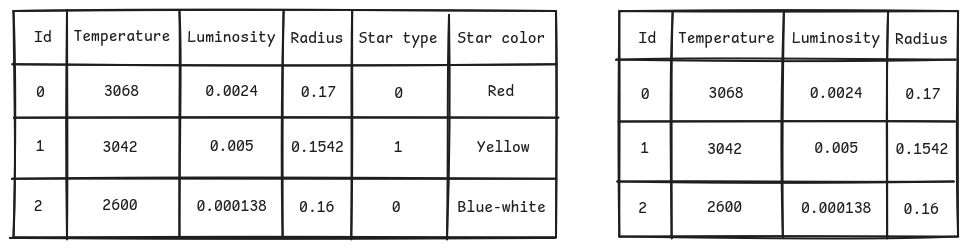
\includegraphics[width=1.0\linewidth]{img/img1.png}
    \caption{Contrapposizione tra dataset con dati etichettati e non-etichettati}
\end{figure}
Come da immagine, la prima tabella possiede alcune colonne in più rispetto alla seconda. Le features aggiuntive esprimono le \textbf{classi} associabili a ciascuna riga, ossia un insieme di valori attribuibili per categorizzare ogni osservazione. \vspace{7pt} \\
Qualora il dataset scelto possieda osservazioni etichettate, ossia ogni sua istanza è associata ad una classe, allora possono essere implementati modelli di apprendimento automatico \textbf{supervisionati}. Essi sfruttano le correlazioni tra i dati e le classi pur di predire l'etichetta associabile per istanze non conosciute. \vspace{7pt} \\
Nonostante, in situazioni reali, è piuttosto complicato possedere un dataset di notevoli dimensioni in cui le informazioni riportate siano tutte etichettate, rendendo impossibile l'impiego di un approccio supervisionato. In queste circostanze è necessario ripiegare su certi algoritmi in grado di ricavare similarità tra i dati, in maniera tale che siano successivamente classificati correttamente. Questo procedimento è condotto da modelli di classificazione \textbf{non-supervisionati}, i quali tentano di compiere tale obiettivo senza l'impiego di informazioni categorizzate preventivamente.

\section{Estrazione e preprocessing dei dati}
\label{2.2}
L'estrapolazione dei dati corrisponde al processo di recupero di informazioni provenienti da fonti eterogenee, spesso non-strutturate, in maniera tale che possano essere convertite in un formato idoneo e facilmente gestibile. Un esempio concreto di quanto riportato, potrebbe avvenire per realtà aziendali che desiderino analizzare la percezione dei propri prodotti da parte dei clienti, basandosi sulle recensioni online. \vspace{7pt} \\
Si consideri un'azienda intenzionata di migliorare i suoi prodotti e a capire quale sia il loro indice di gradimento. In tale ambito, le recensioni costituiscono una fonte ricca di informazioni, ma sono tipicamente espresse in linguaggio naturale, quindi di natura non-strutturata. Per questo motivo, è fondamentale raccogliere un ampio volume di recensioni, riorganizzando i dati contenuti rispetto ad una struttura tabellare, in modo tale che siano agevolmente interpretabili. \vspace{7pt} \\
Il caso di studio della tesi segue sommariamente il titolo esemplificativo. Uno degli obiettivi dell'analisi è ricavare metadati dalla lista di articoli accademici in possesso, sfruttando tecniche di estrazione di informazioni da documenti e sistemi per il recupero dei riferimenti bibliografici. In questo modo, sarà possibile costruire un dataset che potrà essere utilizzato nella fase successiva di classificazione. \vspace{7pt} \\

\subsection{Estrattori di informazioni da documenti}
Il formato \textbf{PDF} è la codifica più diffusa per l'archiviazione e condivisione di documenti digitali. L'estrazione di informazioni da file PDF è essenziale per numerose attività di indicizzazione, recupero di dati e analisi del contenuto. Nonostante il \textbf{Portable Document Format} prediliga un layout visivo di un documento, affinché sia garantito un aspetto coerente su qualsiasi piattaforma software e hardware, include una piccola percentuale di elementi strutturali, i quali rendono la fase di estrapolazione di dati piuttosto complessa e difficile \cite{2023arXiv230309957M}. \vspace{7pt} \\
Nel corso degli anni, sin dall'introduzione del formato, sono state sviluppate diverse soluzioni dedite all'estrazione dei dati, evolvendosi di pari passo al progresso tecnologico: dagli algoritmi rules-based, al machine learning, fino a soluzioni legate a modelli di deep learning. Una fra di esse, la quale ha dimostrato in differenti circostanze ottimi risultati, è la libreria \textbf{GROBID}. \vspace{7pt} \\
GROBID è uno strumento progettato per ricavare informazioni da file PDF di origine accademica, riorganizzandoli in un formato strutturato noto come \textbf{XML/TEI}. \vspace{7pt} \\ 
La conversione della risorsa avviene mediante l'impiego di una sequenza di algoritmi di machine learning, adottando un \textbf{approccio modulare} che tenta di adattarsi alle caratteristiche gerarchiche del documento. Inizialmente sono individuate le macro-aree che contraddistinguono la risorsa, come l'introduzione, i capitoli oppure i paragrafi, per poi estrarne il contenuto. \vspace{7pt} \\ 
Ad ogni iterazione viene attivato un determinato modello di apprendimento automatico, al quale viene assegnato un numero limitato di etichette da associare alle sezioni del file. In questo modo è garantita una chiara separazione dei ruoli e delle funzioni, semplificando l'integrazione di risultati generati da ulteriori algoritmi di machine learning. Pertanto, ogni classificazione confluisce nella fase successiva di etichettatura, definendo un percorso a cascata che porta ad un risultato altamente dettagliato \cite{grobid2024}. \vspace{7pt} \\ 
I modelli di machine learning utilizzati dalla libreria si suddividono in due categorie, quali:
\begin{itemize}
    \renewcommand{\labelitemi}{-}
    \item \textbf{Modelli per riga}. \\
    I modelli della prima tipologia operano per ogni riga che compongano il documento, tendenzialmente impiegati qualora debbano essere definite le sezioni principali della risorsa, assicurando un'elevata velocità di computazione a discapito della qualità della classificazione.
    \item \textbf{Modelli per token}. \\
    I modelli per token estraggono le informazioni che effettivamente contiene il documento. Contrariamente ai modelli precedenti, garantisce un'elevata precisione ma richiede tempi di esecuzione superiori.
\end{itemize}
L'immagine \ref{fig:2.2.2-2.1} rappresenta visivamente l'approccio modulare descritto prima. Ogni singola entità contiene al suo interno una combinazione di algoritmi di \textbf{classificazione} e di \textbf{tokenizzazione}, affinché sia acquisita la porzione di contenuto desiderata. La radice raffigura il \textbf{segmentation model} incaricato di stabilire le sezioni usuali di un articolo scientifico, destinate ai modelli successivi che si occuperanno di ricavarne le informazioni.
\begin{figure}[H]
    \centering
    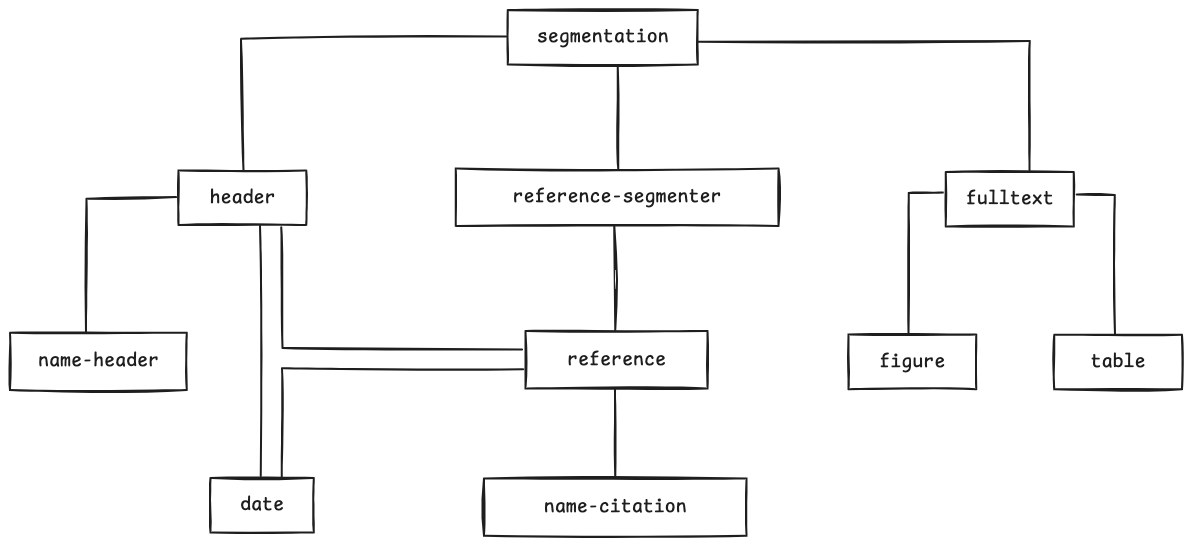
\includegraphics[width=.9\linewidth]{img/img2.png}
    \caption{Raffigurazione dell'approccio modulare di GROBID}
    \label{fig:2.2.2-2.1}
\end{figure} 

\subsection{Sistemi di recupero e gestione dei riferimenti}
La raccolta di metadati inerenti ad articoli scientifici richiede l'accesso a una vasta gamma di risorse informative. Tuttavia, in queste casistiche, occorre utilizzare repository attendibili, che garantiscano la massima accuratezza. Il contesto universitario si distingue per un'ampia varietà di sistemi dedicati al recupero di parametri relativi a pubblicazioni accademiche, noti come \textbf{sistemi di recupero di riferimenti}. \vspace{7pt} \\
Un sistema di recupero di riferimenti è un insieme di strumenti e metodi utilizzati per individuare, raccogliere e organizzare informazioni relative a fonti documentarie, come libri, paper, tesi e altri materiali. Questi sistemi facilitano la ricerca e la gestione delle fonti, garantendo coerenza e precisione nelle citazioni e nelle bibliografie. \vspace{7pt} \\
Nel panorama accademico, è possibile usufruire di un'elevata molteplicità di tali sistemi, ognuno dei quali offre differenti funzionalità volte a facilitare il processo di acquisizione delle risorse, come CrossRef, arXiv, piuttosto che OpenAlex. \vspace{7pt} \\
\textbf{CrossRef} è un'associazione indipendente per la costruzione di tecnologie condivise. La sua missione è quella di migliorare l'accesso alle pubblicazioni scientifiche, attraverso servizi basati su accordi collettivi con editori del settore accademico e professionale \cite{Howells01042006}. \vspace{7pt} \\
La progettazione dell'infrastruttura è architettata con uno scopo ben definito: facilitare la trascrizione delle citazioni all'interno delle pubblicazioni. Ciò avviene mediante l'impiego di \textbf{Digital Object Identifier}, estensione dell'acronimo \textbf{DOI}, identificativi univoci e persistenti di una qualsiasi risorsa digitale riconosciuta. Inoltre, offre numerosi servizi volti all'estrapolazione di metadati inerenti a lavori di ricerca, tra cui una solida \textbf{REST API}, in maniera tale da ottenere il probabile codice univoco una volta fornito  il titolo e la lista di autori del documento. \vspace{7pt} \\
\textbf{OpenAlex} è un catalogo bibliografico che raccoglie un'ampia gamma di risorse e offre una robusta REST API, gratuita e priva di autenticazione, per il recupero di metadati relativi a specifici paper \cite{openalex}. Va sottolineato che la maggior parte delle informazioni reperibili tramite OpenAlex provengono direttamente da CrossRef, il che potrebbe renderlo uno strumento marginale. Nonostante ciò, il suo ruolo è rafforzato dalla rilevazione del database \textbf{Microsoft Academic}, precedentemente riconosciuto come il principale archivio di pubblicazioni provenienti da conferenze.

\subsection{Ulteriori strumenti per la manipolazione di PDF}
\label{2.2.3}
Malgrado l'applicazione di estrattori di dati, alcuni PDF potrebbero non essere compatibili, da cui la potenziale assenza di informazioni associate. Pertanto, possono essere adotatti ulteriori metodi ausiliari, pur di estendere l'analisi condotta ad un bacino più vasto possibile di documenti, tra cui:
\begin{itemize}
    \renewcommand{\labelitemi}{-}
    \item \textbf{Librerie Python}. \\
    Python è uno dei linguaggi di programmazione con il numero maggiore di librerie dedicate alla lettura e manipolazione di PDF. La facilità di sviluppo di questi strumenti rappresenta una valida alternativa per tutti quei documenti incompatibili con estrattori di informazioni. A livello implementativo, l'impiego delle librerie si traduce in una banale operazione di lettura dei documenti: una volta specificato il percorso del file, è restituito un oggetto caratterizzato dall'insieme di tutti i parametri recuperati. Nonostante la varietà di opzioni disponibili, i risultati ottenuti dalle librerie tendono a essere molto simili. Tuttavia, spesso differiscono in base alla velocità di elaborazione e all'accuratezza delle informazioni estratte, differenze che potrebbero influenzare la scelta dello strumento più adatto a seconda delle esigenze implementative. Tra le librerie più utilizzate è possibile citare \textbf{PyPDF} \cite{pypdf2024}, \textbf{PyMuPDF} \cite{pymupdf} e \textbf{PDFPlumber} \cite{pdfplumber}, ognuna contraddistinta da propri punti di forza e di debolezza.
    \item \textbf{Optical Character Recognition (OCR)}. \\
    Qualora l'estrazione di dati sia formalizzata su una collezione di file PDF, occorre considerare l'eventualità che alcuni documenti non siano creati digitalmente, ma realizzati successivamente ad una scansione. A tal proposito, le tecniche di elaborazione descritte fino ad ora potrebbero non garantire gli esiti attesi. Tuttavia, è possibile adoperare meccanismi di Optical Character Recognition, in cui immagini di testo sono convertite in un formato leggibile dalla macchina. Anche in questo contesto, Python offre svariate soluzioni relative a OCR, come \textbf{PyTesseract}. Python-tesseract è un \textbf{wrapper} della libreria Tesseract-OCR sviluppata da Google, progettato per ricavare il contenuto testuale intrinseco a immagini. Per utilizzare il package, è necessario trasformare i PDF in possesso in immagini, procedimento che potrebbe aumentare i tempi di esecuzione. Inoltre, solitamente, vengono attuati diversi filtri volti a migliorare la precisione e la velocità di lettura, modificando la scala di colori dell'immagine: spesso è applicata una gradazione scura, in grado di mettere in risalto il contenuto rispetto allo sfondo.  
\end{itemize}

\subsection{Preprocessing dei dati}
La fase di pre-elaborazione dei dati può influenzare in modo significativo l'esito dei risultati di un modello di machine learning. Il preprocessing svolge un ruolo vitale in qualsiasi operazione di classificazione, poichè migliora la qualità delle informazioni disponibili garantendo una maggiore efficacia e accuratezza degli algoritmi di apprendimento automatico impiegati. \vspace{7pt} \\
Poichè il caso di studio utilizza dati provenienti dal \textbf{linguaggio naturale}, la conversione dell'informazioni testuali in un formato idoneo, le quali per definizione sono disordinate e non-strutturate, rappresenta un passaggio critico. \vspace{7pt} \\
Tendenzialmente, affinché sia migliorata la qualità dei testi, sono implementate determinate tecniche dedite alla pre-elaborazione, suddivise in:
\begin{itemize}
    \renewcommand{\labelitemi}{-}
    \item \textbf{Casefolding}. \\ Il casefolding consiste nella trasformazione di una stringa in minuscolo oppure in maiuscolo, in modo tale da ovviare a circostanze in cui sia dettata l'importanza di una parola in base alla sua forma.
    \item \textbf{Lemmatizzazione}. \\ Le parole articolate all'interno di un discorso possiedono flessioni differenti: i sostantivi variano sintatticamente dal plurale al singolare, mentre i predicati differiscono in base alla forma verbale. Un approccio possibile prevede di uniformare ogni termine, ignorandone la coniugazione, convertendo i nomi al singolare e i verbi all'infinito. In sintesi, ogni parola viene convertita nel suo \textbf{lemma}, ovvero nella sua forma originale.
    \item \textbf{RegEx}. \\ Abbreviazione di \textbf{Regular Expression}, \textbf{RegEx} è uno strumento estramemente potente per la costruzione di pattern di ricerca, impiegati per individuare specifiche sezioni di testo. Il suo caso d'uso principe consiste nella rimozione di parti ritenute superflue di un documento.
    \item \textbf{Stopwords}. \\ Sono categorie di parole che si ripetono con una certa insistenza all'interno di una lingua, come ad esempio gli articoli oppure le congiunzioni, le quali possiedono un valore marginale. L'insieme di questi termini è riconosciuto con la denominazione \textbf{stopwords}, spesso rimosse a priori dal testo. Librerie del calibro di \textbf{NLTK} forniscono insiemi di stopwords in base alla lingua indicata, affinchè possano essere eliminate.
\end{itemize}
L'implementazione delle tecniche richiede una previa operazione di \textbf{segmentazione}, in cui il contenuto di un documento viene scomposto in molteplici entità. Un esempio comune consiste nella \textbf{word tokenization}, dove un determinato elemento \textbf{tokenizer} suddivide un testo nella lista di parole che lo compone.

\section{Modelli di classificazione non-supervisionata}
\label{2.3}
Dalle proprietà del dataset dipendono i modelli di classificazione adoperabili. Se l'analisi condotta dovesse formalizzarsi su una collezione di documenti, da cui l'assenza di dati etichettati, allora sarà possibile usufruire solamente di algoritmi di tipo non-supervisionato. \vspace{7pt} \\
Al fine di categorizzare le informazioni in possesso, possono essere valutate differenti opportunità. Tendenzialmente, modelli non-supervisionati prevedono l'impiego di \textbf{cluster}, ovvero raggruppamenti di istanze simili all'interno di medesimi insiemi. Al tempo stesso, i \textbf{Large Language Models} rappresentano una valida alternativa, dati i continui miglioramenti dimostrati durante l'esecuzione di task in ambito NLP, anche se in questa circostanza è necessario definire a priori le classi che dovranno essere impiegate durante la fase di catalogazione dell'osservazioni. \vspace{7pt} \\
Nei paragrafi seguenti sono illustrate alcune delle classificazioni applicabili, in accordo con quanto anticipato, nel caso in cui il dataset scelto non abbia osservazioni etichettate.

\subsection{Classificazione con Large Language Models}
\label{2.3.1}
La raccolta di informazioni preventivamente etichettate risulta essere piuttosto impegnativa e costosa. Da questa difficoltà è emersa la necessità di sviluppare modelli alternativi, in grado di categorizzare i dati anche in assenza di esempi etichettati, portando così alla diffusione dei sistemi di classificazione \textbf{Zero-Shot} \cite{vajjala2025textclassificationllmera}. \vspace{7pt} \\
Con l'espressione Zero-Shot si intende che la fase di apprendimento del modello si basa esclusivamente sulle conoscenze in possesso, senza che siano fornite informazioni previamente classificate.\vspace{7pt} \\
Tuttavia, dal quadro delineato, emerge l'esigenza di individuare dei modelli che siano in possesso di una vasta gamma di nozioni, spesso riconducibili ai \textbf{Large Language Models (LLM)}. I \textbf{Large Language Models} hanno mostrato notevoli miglioramenti delle proprie prestazioni in differenti task di Natural Language Processing, manifestando capacità sempre più affini alla comprensione del linguaggio naturale, riconosciuti dalla loro discreta abilità di interpretare il significato semantico di un testo \cite{vajjala2025textclassificationllmera}. \vspace{7pt} \\
Sebbene questo approccio abbia i suoi limiti e i modelli circoscritti non eccellono in tutti i compiti di annotazione del testo, differenti ricerche illustrano numerose circostanze in cui LLM possono produrre classificazioni di alta qualità \cite{pangakis2024knowledgedistillationautomatedannotation}. \vspace{7pt} \\
Concludendo, qualsiasi classificazione testuale condotta da Large Language Models deve rispettare due condizioni di primaria importanza, quali:
\begin{itemize}
    \renewcommand{\labelitemi}{-}
    \item \textbf{Valorizzare la qualità dei dati piuttosto che la quantità}. \\
    Dato che modelli LLM basano il loro risultato sul significato semantico del testo, è necessario fornire informazioni che valorizzino la qualità dei dati, magari applicando le stesse operazioni descritte all'interno del Paragrafo \ref{2.2}.
    \item \textbf{Esprimere in maniera concisa la richiesta di classificazione}. \\
    L'interazione con modelli generativi avviene principalmente tramite la formulazione di un \textbf{prompt}, ovvero un testo in linguaggio naturale che specifica un'attività da eseguire. Maggiore è la chiarezza e la precisione della richiesta, più alta sarà la probabilità che il modello di apprendimento automatico restituisca il risultato atteso.
\end{itemize}

\subsection{Classificazione con topic models (BERTopic)}
I convenzionali modelli non-supervisionati impiegano rappresentazioni basate su \textbf{Bag of Words}, in cui un documento viene trasformato in un elenco di parole distinte riportandone il relativo numero di occorrenze. Tuttavia, questo approccio comporta ad una valorizzazione della numerosità dei termini, a discapito della vera relazione semantica che li contraddistingue. \vspace{7pt} \\
In risposta a tale problematica, le tecniche di \textbf{text-embeddings}, in cui le informazioni non-strutturate sono riprodotte in un formato numerico, hanno riconosciuto una rapida espansione senza precedenti, divenendo un elemento chiave all'interno della letteratura. A tal proposito, BERT e le sue varianti hanno dimostrato eccellenti risultati in ambito di \textbf{rappresentazioni vettoriali} di dati testuali, mantenendo un elevato significato semantico \cite{grootendorst2022bertopic}. \vspace{7pt} \\
Nell'immagine seguente sono raffigurati alcuni termini semanticamente simili tra loro. Le rappresentazioni vettoriali delle parole \textbf{wolf} e \textbf{dog} sono posizionate in prossimità, poiché appartengono alla stessa famiglia di canidi. Ciò avviene anche per il vettore \textbf{cat}, dato che assieme a dog sono entrambi animali domestici. Contrariamente, sul lato opposto sono riportati vocaboli che non possiedono alcuna similarità con i vettori illustrati fino ad ora. 
\begin{figure}[H]
    \centering
    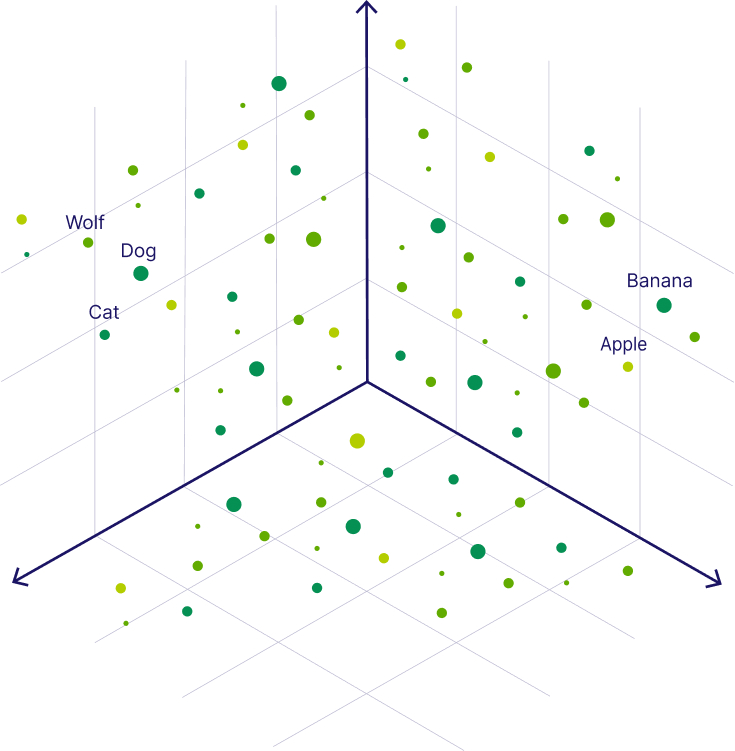
\includegraphics[width=.5\textwidth]{img/img3.png}
    \caption{Raffigurazione vettoriale di informazioni testuali}
\end{figure}
Nonostante i metodi citati possano essere applicati ad una vasta gamma di obiettivi, un possibile scenario d'uso prevede il loro impiego nelle operazioni di \textbf{topic modeling}, finalizzate all'identificazione di temi ricorrenti all'interno di un testo. Un algoritmo in grado di soddisfare una richiesta simile è il modello \textbf{BERTopic}. \vspace{7pt} \\
Il modello genera i topic comuni alla lista di documenti data in ingresso, mediante il conseguimento di tre iterazioni principali.
\begin{itemize}
    \renewcommand{\labelitemi}{-}
    \item \textbf{Conversione dei documenti}. \\
    Il modello inizialmente presuppone che le risorse fornite contengano intrinsecamente temi correlati, in maniera tale che possa dedurre codifiche vettoriali che siano semanticamente confrontabili. La conversione avviene mediante il framework \textbf{SBERT}, il quale permette di trasformare frasi e paragrafi nella propria controparte numerica, utilizzando language models pre-addestrati. I risultati ottenuti sono poi adoperati per raggruppare documenti aventi un significato simile.
    \item \textbf{Raggruppamento dei documenti}. \\
    L'aumento della dimensionalità dei dati causa una minore precisione del quadro delineato nello spazio vettoriale, in cui le distanze differiscono marginalmente tra documenti eterogenei. In queste circostanze è necessario ridurre la dimensione degli embeddings affinché algoritmi di clustering possano operare al meglio delle proprie possibilità.
    \item \textbf{Rappresentazione dei topic}. \\
    Dopo al raggruppamento, ogni cluster è contraddistinto da una serie di possibili topic, rendendo necessario selezionare quelli più pertinenti. Ciò avviene tramite una particolare implementazione della tecnica \textbf{TF-IDF}, utilizzata per valutare la rilevanza di un termine all'interno di un documento, secondo la formula:
    \begin{center}
        $W_t,_d = tf_t,_d \cdot log(\frac{N}{df_t})$
    \end{center}
    dove:
    \begin{itemize}
        \renewcommand{\labelitemi}{-}
        \item \textbf{Term Frequency} ($tf_t,_d$). \\
        Numero di occorrenze di un termine nel documento.
        \item \textbf{Inverse Document Frequency} ($log(\frac{N}{df_t})$). \\
        Misura l'importanza di un termine rispetto all'intera collezione di documenti.
    \end{itemize}
    L'algoritmo BERTopic adotta una procedura simile, ma attuandola a livello di cluster: l'incisività di una parola non è stabilita in base alla completa raccolta di documenti, ma è calcolata impiegando esclusivamente i contenuti presenti all'interno del cluster. Di conseguenza, la formula viene adattata come segue:
    \begin{center}
        $W_t,_d = tf_t,_d \cdot log(1+\frac{A}{df_t})$
    \end{center}
    dove:
    \begin{itemize}
        \renewcommand{\labelitemi}{-}
        \item \textbf{Term Frequency} ($tf_t,_d$). \\
        Immutato rispetto all'equazione precedente.        
        \item \textbf{Inverse Class Frequency} ($log(1+\frac{A}{df_t})$). \\ 
        Determina il peso di un termine rispetto ad una classe di documenti, corrispondente al cluster considerato.
    \end{itemize}
    In sintesi, questa tecnica, nota come \textbf{class-based TF-IDF}, consente di valutare l'importanza delle parole in base a classi di documenti di appartenenza, che in questo contesto sono rappresentate dai cluster individuati in precedenza.
\end{itemize}

\subsection{Classificazione con modelli self-supervised (BART)}
L'apprendimento \textbf{auto-supervisionato} ha raggiunto notevoli traguardi in vari ambiti del Natural Language Processing \cite{DBLP:journals/corr/abs-1910-13461}. Il \textbf{self-supervised learning} è una via di mezzo tra l'approccio \textbf{supervisionato} e \textbf{non-supervisionato} poiché acquisisce in input dati non annotati e li arricchisce con etichette generate autonomamente. \vspace{7pt} \\
I modelli supervised sono in grado di ottenere ottime prestazioni per i compiti per cui sono stati allenati ma non sono in grado di adeguare una generalizzazione degli stessi. Per ricavare le conoscenze necessarie per svolgere nuovi compiti è necessario fornire continuamente nuovi insiemi di dati etichettati, tuttavia spesso non sono presenti o troppo costosi da ricavare. Da questa circostanza è nata la necessità di modelli in grado di accumunare i due aspetti, ovvero comprendere meglio la realtà mediante i dati di training. Il self-supervised è una delle tecniche più promettenti per riuscire ad approssimare tale richiesta.  \vspace{7pt} \\
Il caso d'uso principale per modelli auto-supervisionati prevede l'elaborazione del linguaggio naturale, in totale assenza di esempi etichettati. Infatti, i sistemi self-supervised sono progettati in modo tale che la classificazione delle osservazioni sia dedotta in totale assenza di informazioni previamente categorizzate. \vspace{7pt} \\  
Sebbene l'apprendimento auto-supervisionato vari a seconda dello scenario, i modelli risultanti sono generalmente addestrati seguendo due approcci:
\begin{itemize}
    \renewcommand{\labelitemi}{-}
    \item \textbf{Apprendimento auto-predittivo}. \\ L'apprendimento auto-predittivo addestra un modello affinché possa prevedere parte di un campione di osservazioni date le informazioni rimanenti. I modelli che rientrano in questa categoria sono gli \textbf{Autoencoder}. Un Autoencoder raffigura una rete neurale incaricata di effettuare due azioni successive: inizialmente codifica le variabili in ingresso ricevute, per poi attuare una decodifica volta a ripristinare i dati nella loro forma originale. Ricostituendo le informazioni, i modelli estrapolano una rappresentazione estremamente significativa, poiché permette di apprendere solo le relazioni più importanti che coesistono all'interno del dataset, agevolando in questo modo la possibilità di risolvere problemi non ancora noti.
    \item \textbf{Apprendimento contrastivo}. \\
    I modelli basati sul \textbf{contrastive learning} apprendono la capacità di distinguere coppie di dati che contengano elementi simili, basandosi esclusivamente sulle features estratte dalle osservazioni. La peculiarità di questa tecnica sta nel fatto che non richieda dati etichettati pur di ricavare tali features. I modelli ottenuti sono spesso impiegati per il riconoscimento delle immagini.
\end{itemize}
Proseguendo, è possibile affermare che la letteratura è contraddistinta da una numerosa cardinalità di modelli di intelligenza artificiale addestrati tramite un approccio auto-supervisionato, i quali hanno contribuito alla risoluzione di differenti problematiche in sviariati settori. Uno tra questi, che si è distinto per il significativo impatto nel campo NLP, è l'algoritmo di machine learning \textbf{BART}. \vspace{7pt} \\
BART è un \textbf{pre-trained denoising autoencoder}, ovvero un modello addestrato su un ampio insieme di dati corrotti, progettato per ricostruirli nel loro stato iniziale. Come suggerisce la definizione, utilizza una particolare tipologia di Autoencoder in cui i dati in ingresso non vengono solamente compressi in una rappresentazione più compatta, causando una perdita di informazioni, ma subiscono un'alterazione intenzionale, affinché non coincidano con quelli originali. \vspace{7pt} \\
Dato che si formalizza su paradigmi self-supervised, permette di eseguire task relative al linguaggio naturale per archivi di informazioni prive di etichette. Il modello si dimostra particolarmente efficacie sia per operazioni di generazione di testo ma anche per compiti di comprensione ed interpretazione, capacità che lo rendono un perfetto candidato per attività di classificazione. \vspace{7pt} \\
Tra le funzionalità offerte, consente di realizzare una classificazione testuale secondo il metodo \textbf{Zero-Shot}: forniti i dati e la lista predefinita di classi da associare, restituisce un numero reale compreso tra zero e uno per stabilire il grado di correlazione tra ciascuna osservazione e la collezione di etichette.

\chapter{Sviluppo estrazione dei metadati}
\label{3.0}
D'ora in poi verranno messi in pratica i concetti esposti nel Capitolo \ref{2.0}, concentrando il caso di studio sugli esiti ottenuti dallo sviluppo. \vspace{7pt} \\
Prima di applicare gli algoritmi di classificazione, sono stati creati due dataset contenenti alcuni parametri relativi a un archivio di articoli accademici. Inizialmente i documenti sono stati elaborati per estrarne il contenuto, grazie all'impiego di GROBID e di appositi package (\ref{2.2}). \vspace{7pt} \\
I dati estrapolati sono stati poi inseriti in un lista di oggetti di tipo \textbf{Metadata} (\ref{lst:Metadata}), in modo tale che sezioni degli articoli fossero facilmente manipolabili. Attività che si è rilevata piuttosto utile durante la fase di acquisizione di DOI, ottenuti attraverso le REST API fornite dai principali sistemi di recupero di riferimenti bibliografici. \vspace{7pt} \\
Infine, a partire dalla struttura dati ottenuta, sono stati implementati due dataset, mediante la libreria \textbf{Pandas} di Python, racchiudendo l'insieme di tutte le osservazioni recuperate. La suddivisione in due dataframe avviene per rispondere alle esigenze architetturali dei modelli di apprendimento automatico adoperati.

\section{Passaggi preliminari}
\label{3.1}
Prima di discutere delle varie scelte implementative e degli aspetti tecnici di cui si avvale la tesi, sono illustrate le caratteristiche della collezione di articoli scientifici su cui si concentra il caso di studio presentato, definendo quali di esse possano costituire le features dei dataset circoscritti. \vspace{7pt} \\
Si ricorda che un dataset è una tabella di osservazioni, dove le colonne determinano le features, mentre le righe rappresentano le entità contenute: dal punto di vista matematico un dataset è una matrice di dimensione $N \times d$. \vspace{7pt} \\
Dopodiché, sono elencati i metadati che costituiscono i domini dei dataframe, riportando una breve descrizione per ognuno di essi.

\subsection{Progettazione del dataset}
\label{3.1.1}
Il lavoro di questa tesi nasce da una precedente pubblicazione scientifica, in cui un archivio di paper è stato utilizzato per identificare parole chiave e argomenti ricorrenti al loro interno, tramite l'impiego di strumenti di machine learning \cite{Borghesi_2024}. \vspace{7pt} \\
A tal proposito, la collezione è composta da $1952$ documenti, in formato PDF, diffusi dal $1950$ fino al $2021$, focalizzati sul parallelismo tra il mondo degli scacchi e l'evoluzione dell'intelligenza artificiale, in particolare di quanto quest'ultima abbia influito in ambito computer chess. \vspace{7pt} \\
Proseguendo, uno degli obiettivi del caso di studio prevede lo sviluppo e il miglioramento del processo di acquisizione dei dati dallo stesso archivio di paper. Pertanto, ciascuna pubblicazione è stata sottoposta ad un processo di estrapolazione di informazioni, affinché il contenuto ricavato fosse elaborato e racchiuso all'interno di un dataframe, definendo in questo modo le variabili in ingresso necessarie per adeguare certi algoritmi di apprendimento automatico (\ref{4.0}). \vspace{7pt} \\
È importante sottolineare che il flusso implementativo è stato progettato con lo scopo di garantire totale indipendenza tra la costruzione del dataset e l'archivio di file PDF. Questo approccio consente alla logica sviluppata di essere flessibile e adattabile, permettendo di applicarla non solo al caso descritto, ma a qualsiasi raccolta di articoli scientifici, indipendentemente dall'ambito da cui provengano. \vspace{7pt} \\
All'interno della tabella sottostante, sono introdotti i metadati acquisiti per ciascun file della raccolta, scelti per costituire la lista di domini degli insiemi di dati.
\begin{table}[H]
    \begin{tabularx}{\textwidth}{|c|X|X|}
            \hline
            \small 1. & \small \textbf{DOI - (Digital Object Identifier)} & \small Identificativo univoco e persistente di una qualsiasi risorsa digitale \\
            \hline
            \small 2. & \small \textbf{Title} & \small Titolo dell'articolo scientifico \\
            \hline
            \small 3. & \textbf{Author} & \small Autore o lista di autori che abbiano partecipato alla stesura dell'articolo scientifico \\
            \hline
            \small 4. & \small \textbf{Keywords} & \small Lista delle parole chiave più significative relative all'articolo scientifico \\
            \hline
            \small 5. & \small \textbf{Abstract} & \small Riassunto dell'articolo scientifico privo di interpretazioni o critiche sui temi trattati \\
            \hline
            \small 6. & \small \textbf{Introduction} & \small Introduzione dell'articolo scientifico memorizzata nella sua interezza \\
            \hline
    \end{tabularx}
\end{table}

\subsection{Progettazione di classi ausiliare}
Data l'elevata numerosità di paper in formato PDF, sono state implementate alcune classi di supporto in maniera tale da facilitare la fase di estrazione di dati. L'impiego di classi ausiliare, come da titolo esemplificativo, si è rilevato piuttosto utile durante il flusso implementativo, in particolare per il recupero di DOI: le richieste presentate alle REST API, esigono la concatenazione del titolo e della lista di autori dell'articolo scientifico affinché sia ricevuto l'identificativo desiderato. \vspace{7pt} \\
Lo snippet di codice presentato definisce la classe \textbf{Metadata}, in cui ogni istanza raffigura uno specifico documento. 
\begin{lstlisting}[language=python, label=lst:Metadata, caption=Classe Metadata]
class Metadata:
    def __init__(self, DOI: str, path: str, title: str, author: Author | ...):
        self.DOI = DOI
        self.path = path
        self.title = title
        self.author = author
        self.keyword = keyword
        self.abstract = abstract
        self.introduction = introduction

    def get_dict(self) -> Dict[str, Dict[str, str | List[Author] | None]]:
        return {
            self.path: {
                "DOI": self.DOI,
                "Title": self.title,
                "Author": [item.to_unique() for item in self.author],
                "Keyword": self.keyword,
                "Abstract": self.abstract,
                "Introduction": self.introduction
            }
        }
\end{lstlisting}

\section{Estrapolazione delle informazioni}
La preponderanza di PDF ha preteso l'utilizzo di strumenti appositi per la conversione delle risorse in un formato facilmente manipolabile. Nonostante Python sia caratterizzato da numerosi package dedicati alla lettura di file PDF, in alcune circostanze i risultati non sono attendibili. Infatti, la maggior parte delle librerie, alcune di esse definite nel Paragrafo \ref{2.2.3}, hanno riscontrato stesse problematiche relative all'estrazione di dati, tra cui: mancato o erroneo riconoscimento delle sezioni qualora il contenuto dell'articolo fosse disposto in due colonne, incompletezza dei metadati e assenza di informazioni per documenti ottenuti tramite scansione. \vspace{7pt} \\
Da queste difficoltà è emersa la necessità di ripiegare su ulteriori sistemi. Sebbene le tecniche precedenti garantissero una maggiore velocità di esecuzione, GROBID ha estrapolato il contenuto della maggior parte delle risorse presenti nell'archivio. \vspace{7pt} \\
La scelta implementativa è ricaduta sulla combinazione complessiva degli strumenti citati, in modo tale che l'analisi fosse realizzata su uno spettro più ampio possibile. Medesima decisione è stata adeguata per il recupero dei riferimenti bibliografici. CrossRef ha fornito il numero maggiore di riferimenti, ma alcuni articoli risultano assenti nella sua infrastruttura. Per questa ragione, sono state integrate ulteriori REST API specializzate per il recupero di fonti bibliografiche.

\subsection{Lettura tramite GROBID}
\label{3.2.1}
La conversione di documenti in un formato strutturato avviene abilitando il server GROBID. Per avviare il servizio, è possibile usufruire di alcune \textbf{immagini Docker} preconfigurate oppure installare integralmente il software tramite \textbf{Gradle}, anche se questa opzione richiede una previa installazione di una JDK. Una volta attivato, il server sarà raggiungibile alla porta $8070$ del dispositivo, consentendo di verificare il corretto funzionamento della libreria. \vspace{7pt} \\
Dal punto di vista implementativo, è stata adottata la prima soluzione, in cui Docker ha garantito un'elevata facilità di deployment e ha permesso di utilizzare i modelli di machine learning senza importare alcuna dipendenza software. \vspace{7pt} \\
Il team di sviluppo ha fornito due immagini Docker, le quali differiscono in base all'accuratezza della trasformazione e alla velocità di computazione. A tal proposito, è stata preferita l'impostazione più leggera, sacrificando parte della precisione per ottenere tempi di elaborazione più rapidi: sul computer in cui il codice è stato eseguito, la conversione dei file ha richiesto poco più quattro ore.
\begin{lstlisting}[language=python, caption=Conversione di documenti PDF in file XML/TEI]
from grobid_client.grobid_client import GrobidClient

try:
    grobid_client = GrobidClient(config_path="../config.json")
    grobid_client.process(
        "processFulltextDocument",
        input_dir,
        output_dir,
        n=10
    )        
except requests.exceptions.ConnectionError as e:
    print("Connection error during Grobid processing: ", e)
except Exception as e:
    print("Error during Grobid processing: ", e)\end{lstlisting}
Il codice illustra il processo di trasformazione dei documenti, memorizzati all'interno di una determinata cartella. Il passaggio iniziale consiste nella creazione di un \textbf{client} in grado interagire con il servizio abilitato e di stabilire il momento in cui debba essere avviata la conversione. \vspace{7pt} \\
Prima di procedere, occorre sottolineare l'importanza del file JSON dato in ingresso all'istanza della classe \textbf{GrobidClient}. Il file di configurazione possiede alcune proprietà personalizzabili, sintetizzate in:
\begin{itemize}
    \renewcommand{\labelitemi}{-}
    \item \textbf{grobid\_server}: indica il Uniform Resource Locator dove il server sarà raggiungibile.
    \item \textbf{batch\_size}: descrive la dimensione del thread pool impiegato dal \textbf{ThreadPoolExecutor}, determinando il numero massimo di flussi di esecuzione gestiti internamente. La documentazione consiglia di non variare il valore di default, dato che rappresenta un numero sufficientemente alto per garantire un'elaborazione efficiente, ma non eccessivo, in modo tale che sia preservata la memoria della macchina.
    \item \textbf{sleep\_time}: definisce il tempo di attesa prima di inviare una nuova richiesta a GROBID quando il server segnala che tutti i suoi thread sono attualmente occupati. Il tempo di attesa varia a seconda alla tipologia di conversione: nel caso in cui il documento sia convertito nella sua interezza, noto come \textbf{proccessFullTextDocument}, è consigliato un intervallo di 5-10 secondi, mentre per attività di \textbf{processHeaderDocument} è sufficiente un tempo di attesa pari a 2 secondi.
\end{itemize}
Al termine della conversione, il risultato restituito consiste in un insieme di risorse di estensione \textbf{XML/TEI}. I pattern ripetitivi dei tag XML hanno facilitato l'estrapolazione delle informazioni desiderate, utilizzando la libreria \textbf{BeatifulSoup}. \vspace{7pt} \\
Il package è progettato per analizzare contenuti basati su linguaggi di markup, organizzandoli in una struttura dati ad albero. Questo permette di accedere agevolmente alle differenti entità che compongano un articolo scientifico, ognuna delle quali dispone di propri parametri, a seconda degli attributi e del corpo dell'elemento.
\begin{figure}[H]
    \centering
    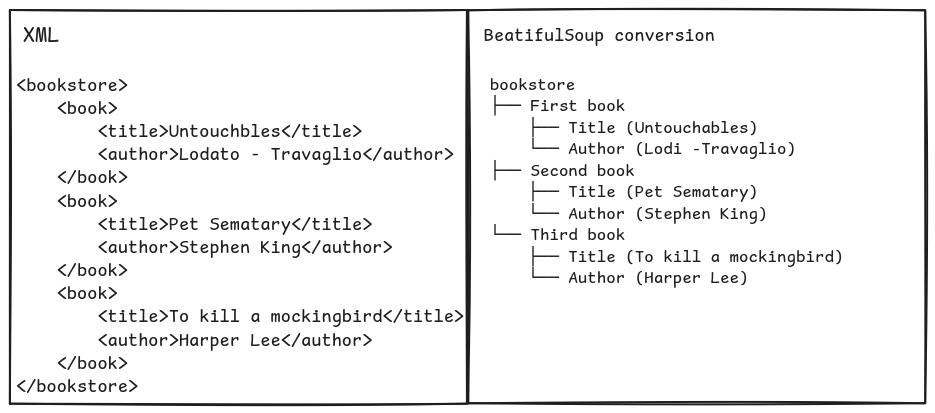
\includegraphics[width=.7\textwidth]{img/img4.png}
    \caption{Organizzazione dei tag XML secondo una struttura ad albero}
    \label{fig:3.2.1-3.1}
\end{figure}
Di seguito è definito lo snippet di codice che si avvale di BeatifulSoup per ricavare i metadati necessari. Qualora non vi sia corrispondenza tra la struttura dati e la lista di tag XML data in ingresso, è restituito un valore \textbf{None}.
\begin{lstlisting}[language=python, caption=Estrazione dell'informazioni tramite BeatifulSoup]
from bs4 import BeautifulSoup

def extract_content(soup: BeautifulSoup, tags: List[str]) -> str:
    try:
        element = soup.find(tags[0])

        for tag in tags[1:]:
            element = element.find(tag)

        return element.contents[0]
    except Exception:
        return None\end{lstlisting}
Le informazioni ricavate sono inserite iterativamente all'interno di una lista di oggetti di tipo \textbf{Metadata} (\ref{lst:Metadata}), per poi essere adoperate durante la fase di acquisizione dei riferimenti bibliografici.

\subsection{Lettura tramite librerie Python}
Sebbene GROBID abbia garantito ottimi rendimenti, una porzione di risorse dell'archivio non fu compatibile con il servizio, data la conversione in file XML/TEI carenti di contenuti. Per non perdere informazioni preziose si è deciso di impiegare ulteriori librerie Python dedicate alla lettura di file PDF, nella speranza di raccimolare qualche dato aggiuntivo. \vspace{7pt} \\
A partire dalla lista di oggetti di tipo Metadata, introdotta nel Paragrafo \ref{3.2.1}, sono stati individuati gli articoli privi di parametri. I documenti circoscritti sono stati assegnati al modulo \textbf{PDFReader} del package \textbf{PyPDF}, in maniera tale che fosse possibile accedere alle proprietà dell'istanza successivamente alla lettura dei file.
\begin{lstlisting}[language=python, caption=Lettura dei documenti PDF tramite la libreria PyPDF]
pattern = (r"(^.*)?.grobid")

def retrieve_missing_metadata(list_metadata: List[Metadata]):
    for metadata in list_metadata:
        if metadata.title is None or len(metadata.author) == 0:
            pdf_path = re.search(
                pattern,
                metadata.path
            ).group(1) + ".pdf"

            try:
                _pdfreader = PdfReader(input_dir + pdf_path).metadata
            except Exception:
                pass
             
            title = _pdfreader.title or None
            author = _pdfreader.author or []

            _.title = title
            _.path = pdf_path
            _.author = define_authors(author)\end{lstlisting}
Nonostante siano state valutate differenti librerie, è stata implementato un singolo package. La scelta è stata dettata dal fatto che gli esiti ottenuti dalle molteplici librerie non variavano significativamente, distinguendosi principalmente per la velocità di esecuzione. Pertanto, si è optato per una soluzione che garantisse un miglior compromesso tra facilità di sviluppo e prestazioni.

\subsection{Recupero di riferimenti bibliografici (CrossRef)}
\label{3.2.3}
Completata la prima fase di estrazione dei dati, il passaggio consecutivo si concentra sul recupero dei riferimenti bibliografici mediante apposite REST API. La lista di metadati elaborata fino a questo punto, contiene istanze della classe Metadata prive di Digital Object Identifier (DOI). Affinché gli identificativi digitali possano essere acquisiti, occorre interrogare apposite infrastrutture dedicate alla gestione delle fonti documentarie. \textbf{CrossRef} rappresenta in questo contesto l'architettura principale a cui rivolgersi, dato l'elevato ammontare di articoli scientifici presenti al suo interno. \vspace{7pt} \\
L'organizzazione mette a disposizione una \textbf{Web API} da cui ottenere le informazioni desiderate. Inoltre, sono presenti wrapper Python che ne semplificano l'interazione, permettendo di inviare delle query e di gestire le risposte in modo più agevole. In termini di sviluppo, tra le differenti opzioni, la scelta è ricaduta sul package \textbf{crossref}. \vspace{7pt} \\
L'implementazione non ha comportato significativi sacrifici: una volta formulata la richiesta HTTP è inviata all'API di CrossRef, concatenando il titolo e la lista di autori del paper circoscritto. Ottenuta la risposta, in base allo \textbf{Status Code}, sono elaborati e confrontati i dati ricevuti.
\begin{lstlisting}[language=python, caption=Recupero di riferimenti bibliografici tramite CrossRef]
import time
import requests

from crossref.restful import Works

work = Works()
def send_crossref_request(title: str, list_authors: List[str]) -> str:
    url_request = work.query(
        bibliographic=title,
        author=get_authors_string(list_authors)
    ).url
    
    time.sleep(2)

    try:
        response = requests.get(url_request)

        match response.status_code:
            case 200:
                content = response.json()
                message = content.get("message")

                items = message.get("items")
                for item in items:
                    if similar(title, item["title"][0]) > 0.5:
                        return item["DOI"]
                                                                
                    continue
            case 400:
                print("Error during request to CrossRef: Bad Request")
            case _:
                print("Error during request to CrossRef: WTH")
    except Exception as e:
        print("Error during request to CrossRef:", e)\end{lstlisting}
I dati restituiti sono in formato JSON, pertanto, come riportato dall'esempio, è stato necessario recuperarne il contenuto per poi accedere direttamente alle key interessate. Per ogni potenziale corrispondenza è stata attuata una funzione di similarità, incaricata di calcolare la percentuale di somiglianza rispetto a due stringhe date in input. Solamente nel caso in cui la percentuale superi la soglia minima, i metadati associati sono considerati attendibili.
\begin{lstlisting}[language=python, caption=Calcolo della similarità tra due stringhe]
from difflib import SequenceMatcher

def similar(str_1: str, str_2: str) -> float:
    return SequenceMatcher(None, str_1, str_2).ratio()\end{lstlisting}

\subsection{Controllo della validità dei metadati recuperati}
\label{3.2.4}
Per sincerarsi dell'attendibilità dei metadati ricavati, è stato compiuto lo stesso processo ma in senso opposto, ovvero a partire dai DOI, interrogando l'API di CrossRef, sono stati nuovamente recuperati il titolo e gli autori di ciascun paper affinché fossero confrontati con quelli già in possesso. In questo modo si è avuta la possibilità di accertarsi della validità delle informazioni acquisite. \vspace{7pt} \\
I risultati emersi dai vari esperimenti hanno evidenziato che la maggior parte delle risorse sono corrette, se non per una piccola porzione di documenti. Esiti ottenuti utilizzando la stessa funzione di similarità introdotta nella sezione precedente (\ref{3.2.3}), focalizzando il confronto di somiglianza tra i titoli e gli abstract degli articoli scientifici.
\begin{table}[H]
    \centering
    \begin{tabular}{lcc}
        \toprule
        \textbf{Categoria} & \textbf{Numero di articoli} & \textbf{Percentuale} \\
        \midrule
        Articoli & $1952$ & $100\%$ \\
        \hline
        Articoli letti & $1770$ & $91\%$ \\
        \hline
        Articoli recuperati & $1131$ & $64\%$ \\
        Articoli non recuperati & $639$ & $36\%$ \\
        \hline
        Articoli recuperati & $1131$ & $64\%$ \\
        \hline
        Articoli attendibili & $944$ & $83\%$ \\
        Articoli non attendibili & $187$ & $17\%$ \\
        \bottomrule
    \end{tabular}
    \caption{Tabella contenente gli esiti della fase di estrazione di dati}
\end{table}
In particolare, la funzione assegna un punteggio di similarità tra due stringhe date in ingresso. In base al valore attribuito, è possibile determinare se la correlazione tra il documento in possesso rispetto a quello individuato tramite la REST API è valida o meno. Qualora il punteggio sia inferiore a una soglia minima di $0.6$, le informazioni recuperate sono considerate non attendibili. \vspace{7pt} \\
Concludendo, come indicato dalla tabella, il $9\%$ dei file non è stato leggibile e, di conseguenza, non sono stati nemmeno estratti i metadati associati. Questa problematica è dovuta principalmente al fatto che alcuni PDF della raccolta sono stati ottenuti tramite scansione, piuttosto che creati digitalmente. Pertanto, la qualità del testo contenuto nei documenti non è sufficientemente trattabile dai sistemi di estrazione automatica, impedendo una lettura adeguata e scoraggiando l'estrapolazione delle informazioni.  

\subsection{Recupero di riferimenti bibliografici (OpenAlex, arXiv)}
Il Paragrafo \ref{3.2.4} ha evidenziato l'assenza di alcuni metadati, nonostante CrossRef rappresenti l'infrastruttura contenente il numero maggiore di fonti documentarie. Per questa ragione, sono stati impiegati ulteriori strumenti che offrissero servizi dedicati al recupero dei riferimenti bibliografici, pur sempre inerenti all'ambito accademico. In particolare, sono state sfruttate le REST API fornite da: 
\begin{itemize}
    \renewcommand{\labelitemi}{-}
    \item \textbf{OpenAlex}. \\
    La decisione di utilizzare OpenAlex è stata motivata dal riconoscimento del suo database come uno degli archivi più completi e autorevoli di conferenze scientifiche, successivamente alla rilevazione della base di dati Microsoft Academic. Il sistema mette a disposizione un wrapper Python dell'API, con lo scopo di facilitarne l'interazione, denominato \textbf{PyAlex}.
    \item \textbf{arXiv}. \\
    L'adozione di arXiv è dovuta alla stretta analogia dell'informazioni memorizzate nell'infrastruttura rispetto alla collezione di file PDF su cui si basa il caso di studio. Poiché l'archivio del repository raccoglie risorse relative alle scienze naturali e matematiche, vi è una maggiore probabilità di individuare una corrispondenza con i paper in possesso, dato che si concentrano sull'evoluzione dell'intelligenza artificiale. Come avviene per OpenAlex, il sistema offre un wrapper Python dell'API per semplificare la fase di acquisizione.
\end{itemize}
Esposte le motivazioni, sono presentati gli snippet di codice per interrogare le API in questione. La logica di sviluppo, rispetto a CrossRef, non varia significativamente, a parte la formulazione delle richieste HTTP. \vspace{7pt} \\
OpenAlex organizza la banca dati suddividendola in differenti \textbf{entità} e stabilendo le connessioni fra di esse. A livello implementativo, è quindi necessario individuare quale entità possa soddisfare la richiesta. In questo contesto, dato l'utilizzo di articoli scientifici, è stato adottato il modulo \textbf{Works}, che raccoglie tutti i documenti accademici memorizzati, tra cui tesi, libri, riviste e dataset. Una nota negativa di tale approccio, è dovuta all'impossibilità di specificare gli autori dell'articolo, definendo una minore precisione di ricerca.
\begin{lstlisting}[language=python, caption=Recupero di riferimenti bibliografici tramite OpenAlex]
import pyalex

def split_url(url: str) -> str:
    tokens = url.split("/")
    return tokens[-2] + "/" + tokens[-1]

for key, value in dict_missing_metadata.items():
    try:
        _title = value.get("Title")

        works = pyalex.Works().search_filter(title=value.get("Title")).get()

        for work in works:
        
            # Key "doi" in the response contains the paper's DOI as URL
            doi = work["doi"]
            title = work["title"]
            if doi is not None and similar(title, _title) > 0.7:
                dict_missing_metadata[key]["DOI"] = split_url(doi)
                break
    except Exception as e:
        continue
\end{lstlisting}
Contrariamente, \textbf{arxiv} permette di combinare i due parametri. Dopo aver istanziato un oggetto Client, incaricato di gestire la connessione con il server remoto, viene effettuata una ricerca all'interno del repository, formalizzando una query abbinando il titolo e la lista di autori dell'articolo. I risultati della ricerca vengono iterati in modo tale che siano individuate potenziali corrispondenze.
\begin{lstlisting}[language=python, caption=Recupero di riferimenti bibliografici tramite arXiv]
import arxiv

arxiv_client = arxiv.Client()
for key, value in dict_missing_metadata.items():
    _title = value["Title"]
    _author = " ".join(value["Author"])

    search = arxiv.Search(query=f"au:{_author} AND ti:{_title}")

    for result in arxiv_client.results(search):
            try:
                if similar(result.title, _title) > 0.7:  
                    print(result.pdf_url) 
            except Exception:
                continue
\end{lstlisting}
Concludendo, in entrambi i casi, i DOI associati sono ritenuti attendibili solamente se sorpassata la soglia minima di similarità tra le risorse in possesso e quelle ricavate. Malgrado l'applicazione di ulteriori Web API, sono stati recuperati un totale di $6$ fonti bibliografiche, testimoniando quindi la scarsa reperibilità dei documenti mancanti.

\section{Costruzione dei dataset}
In questa sezione viene illustrato lo sviluppo dei dataset, che contengono le osservazioni che verranno utilizzate dagli algoritmi di machine learning nel prossimo capitolo (\ref{4.0}). \vspace{7pt} \\
Dopo aver recuperato la lista di metadati, sono state estratte le features destinate ai dataframe, i quali condividono gli stessi domini presentati nel Paragrafo \ref{3.1.1}. Sono stati realizzati due insiemi di dati per distinguere le informazioni in base ai modelli di classificazione impiegati, attuando a seconda delle circostanze una previa fase di preprocessing. \vspace{7pt} \\
Nel caso di modelli di linguaggio naturale, che si formalizzano sulla comprensione e interpretazione di informazioni testuali, è stato preferito mantenere le risorse nel loro formato originale. Viceversa, per gli algoritmi che richiedono rappresentazioni vettoriali delle variabili in ingresso, sono state adeguate delle operazioni di pre-elaborazione, mirate a migliorare la qualità dei dati e a garantire una maggiore efficacia durante l'etichettatura.
\begin{lstlisting}[language=python, caption=Creazione del primo dataset]
import pandas

data = {
    "DOI": [metadata.DOI for metadata in list_metadata],
    "Title": [metadata.title for metadata in list_metadata],
    "Keywords": [metadata.keyword for metadata in list_metadata],
    "Abstract": [metadata.abstract for metadata in list_metadata],
    "Introduction": [metadata.intro for metadata in list_metadata]
}

df_not_cleaned = pandas.DataFrame(data=data).dropna(
    subset=["DOI", "Title", "Abstract"]
)
df_not_cleaned.head()
\end{lstlisting}
\begin{figure}[h]
    \centering
    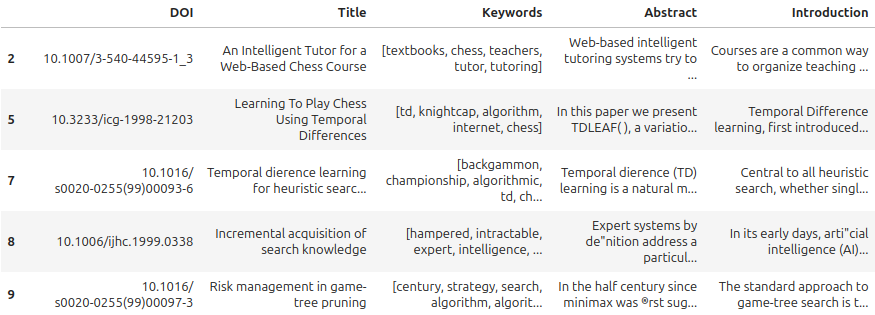
\includegraphics[width=1.0\textwidth]{img/img5.png}
    \caption{Raffigurazione del primo dataset}
    \label{fig:3.3-3.2}
\end{figure}
Al termine della computazione, il dataset ha generato una matrice di dimensione:
\begin{center}
    $N\times d = 1131 \times 5$
\end{center}
dove $N$ è il numero di righe, mentre $d$ rappresenta la cardinalità delle colonne. Questo insieme di dati è utilizzato esclusivamente per modelli di linguaggio naturale. \\
Per il secondo dataset è stata implementata la stessa logica di sviluppo, ma applicando una funzione dedicata alla pre-elaborazione della risorsa data in input. Il preprocessing effettuato sui testi, appartenenti agli articoli scientifici dell'archivio, è sintetizzabile nei seguenti passaggi:
\begin{itemize}
    \renewcommand{\labelitemi}{-}
    \item \textbf{Traduzione in inglese}. \\
    Dopo una breve analisi, sono emersi alcuni documenti della raccolta scritti in lingue differenti. Per tale ragione, affinché sia garantita un'omogeneità dei dati, sono stati tradotti in inglese.
    \item \textbf{Conversione del testo in minuscolo}. \\
    Il testo è convertito in minuscolo, evitando in questo modo casi in cui sia stabilita l'importanza di una parola in base alla sua forma.
    \item \textbf{Tokenizzazione}. \\
    L'informazione testuale è suddivisa nella lista di parole che la compone, rimuovendo articoli, congiunzioni e \textbf{stopwords}. Per la suddivisione in ciascuna parola, è stato impiegato un \textbf{tokenizer} implementato mediante la libreria \textbf{RegexTokenizer}.
    \item \textbf{Lemmatizzazione}. \\
    Ciascuna parola individuata nello step precedente, viene convertita nella sua forma originale, ignorando coniugazione verbali e convertendo i sostantivi al singolare.
\end{itemize}
\begin{lstlisting}[language=python, caption=Preprocessing delle informazioni testuali]
from langdetect import detect
from nltk.stem import WordNetLemmatizer
from nltk.tokenize import RegexpTokenizer
from deep_translator import GoogleTranslator

lemmatizer = WordNetLemmatizer()
tokenizer = RegexpTokenizer(r"[a-zA-Z]+")

def preprocess_field(field: str) -> List[str]:
    try:
        if detect(field) != "en":
            field = GoogleTranslator(source="auto", target="en").translate(field)

        text = field.lower()
        tokens = tokenizer.tokenize(text)

        tokens = [token for token in tokens if len(token) > 2]
        tokens = [token for token in tokens if token not in set_stopwords]

        return [lemmatizer.lemmatize(token) for token in tokens]
    except Exception:
        return [" "]
\end{lstlisting}
\begin{figure}[H]
    \centering
    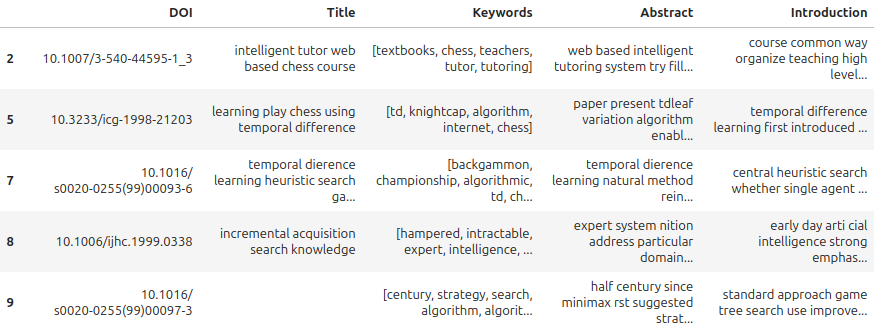
\includegraphics[width=1.0\textwidth]{img/img6.png}
    \caption{Raffigurazione del secondo dataset}
    \label{fig:3.3-3.3}
\end{figure}
Il dataframe circoscritto possiede la stessa dimensione del dataset precedente, a differenza del fatto che le istanze raccolte al suo interno sono successive alle operazioni di pre-elaborazione citate.

\subsection{Considerazioni sui dataset ottenuti}
Quest'ultimo paragrafo del $\ref{3.0}^{\circ}$ Capitolo, riassume la fase di estrazione di informazioni dalla collezione di documenti, focalizzandosi sui metadati ottenuti. \vspace{7pt} \\
Uno degli obiettivi del caso di studio, prevede la costruzione di un dataset in cui sia valorizzata la qualità dei dati piuttosto che la quantità reperibile, sperando che questo processo possa giovare alla classificazione degli articoli da parte di tecniche di apprendimento automatico. Per questa principale ragione, i dataframe ottenuti contengono un numero minore di osservazioni rispetto alla cardinalità delle pubblicazioni scientifiche racchiuse all'interno dell'archivio. \vspace{7pt} \\
La combinazione di GROBID e di librerie Python per la lettura di file PDF si è dimostrata una scelta corretta. Infatti, è stato possibile accedere al contenuto di $1770$ paper su un totale di $1952$. Tuttavia, gli stessi risultati non sono stati raggiunti durante il recupero dei riferimenti bibliografici, poiché è stato possibile ricavare una somma complessiva di Digital Object Identifier (DOI) pari a $1131$, di cui alcuni, come descritto nella sezione \ref{3.2.4}, non sono stati considerati attendibili. Nonostante la mancata correlazione, tali entità sono state preservate all'interno dei dataset, dato che sono contraddistinte sia dal titolo che dall'abstract del lavoro di ricerca. \vspace{7pt} \\
Di seguito, è presentata una tabella contenente tutti i parametri riepilogativi, confrontati con il numero totale di documenti utilizzati durante l'analisi. La percentuale è rapportata rispetto alla cardinalità complessiva degli articoli.
\begin{table}[H]
    \centering
    \begin{tabular}{lcc}
        \toprule
        \textbf{Categoria} & \textbf{Numero di articoli} & \textbf{Percentuale} \\
        \midrule
        Articoli & $1952$ & $100\%$ \\
        \hline
        Articoli letti & $1770$ & $91\%$ \\
        Articoli con titolo & $1736$ & $89\%$ \\
        Articoli con keywords & $1323$ & $68\%$ \\
        Articoli con titolo e keywords & $1312$ & $67\%$ \\
        \bottomrule
    \end{tabular}
    \caption{Tabella contenente i parametri riepilogativi della fase di estrazione}
\end{table}

\chapter{Esperimenti con tecniche di classificazione}
\label{4.0}
Il passaggio finale del caso di studio prevede di classificare i metadati acquisiti durante la fase di estrazione (\ref{3.0}), mediante l'applicazione di specifiche tecniche di machine learning. L'impiego degli algoritmi di apprendimento automatico, descritti nel Paragrafo \ref{2.3}, avviene per soddisfare la richiesta di categorizzazione degli articoli dell'archivio. \vspace{7pt} \\
A causa dell'assenza di classi predefinite associabili alle osservazioni raccolte, è emersa l'esigenza di selezionare alcune \textbf{etichette}, affinché includessero temi discussi dai documenti della collezione. \vspace{7pt} \\
Complessivamente, i modelli di classificazione sono stati implementati secondo un approccio Zero-Shot, volto a riconoscere pattern ripetitivi all'interno dell'entità date in ingresso, basandosi esclusivamente sulle conoscenze in possesso. A tal proposito, sono stati adoperati modelli \textbf{pre-addestrati} e \textbf{non-supervisionati}, data la mancanza di dati annotati. \vspace{7pt}\\
I paragrafi successivi evidenzieranno la capacità marginale delle tecniche di machine learning durante la classificazione dei paper, nonostante sia stata condotta un'attività preliminare di estrazione dei dati incentrata sulla qualità delle informazioni piuttosto che sulla quantità disponibile.

\section{Selezione delle etichette}
\label{4.1}
Problemi di classificazione testuale richiedono una lista di categorie da assegnare ad una collezione di dati. In base alle osservazioni contenute nel dataset, è possibile affermare la presenza di label o meno. Qualora l'insieme di dati racchiuda informazioni etichettate al suo interno, allora saranno presenti una o più classi, contrariamente saranno assenti per risorse non-etichettate. \vspace{7pt} \\
Per definizione, usufruire di un archivio di documenti comporta alla manipolazione di dati non-strutturati e, a maggior ragione, alla mancanza di etichette. Dal quadro delineato, emerge l'esigenza di identificare un insieme di classi adoperabili durante la fase di annotazione. \vspace{7pt} \\
Il flusso implementativo che ha caratterizzato il caso di studio ha permesso di realizzare un sistema completamente svincolato dalle etichette scelte, garantendo la capacità di compiere attività di classificazione indipendentemente dai topic selezionati. Questo approccio ha introdotto un livello di astrazione che consente di separare le entità da classificare e le etichette, facilitando il processo di aggiornamento delle categorie mantenendo le stesse osservazioni. \vspace{7pt} \\
Sfruttando alcuni Large Language Model e conoscenze diffuse in ambito computer chess, sono stati selezionati alcuni topic attribuibili alla raccolta di metadati. È bene precisare che le categorie selezionate non pretendono di essere le uniche utilizzabili, ma rappresentano un solido punto di partenza per valutare la bontà delle classificazioni prodotte dai modelli di machine learning presentati. \vspace{7pt} \\
In particolare, le categorie impiegate appartengono a tre differenti macro-insiemi, quali:
\begin{itemize}
    \renewcommand{\labelitemi}{-}
    \item \textbf{Etichette ricavate tramite LLM}. \\
    Le categorie fornite interrogando ChatGPT sono rappresentate da un elenco suddiviso in due livelli distinti: il primo livello definisce il tema generale, mentre il secondo livello approfondisce argomenti più specifici.
    \begin{table}[H]
        \begin{tabularx}{\textwidth}{|c|X|X|}
            \hline
            \small \textbf{\#} & \small \textbf{Etichette di Primo livello} & \small \textbf{Etichette di Secondo livello} \\
            \hline
            \small 1. & \small Algorithmic Approaches & \small Search Techniques, Heuristics and Evaluation, Machine Learning \\
            \hline
            \small 2. & \small Architectural Designs & \small Chess Engines, Distributed Systems, Hardware \\
            \hline
            \small 3. & \small Game Stages & \small Opening Play, Middlegame Play, Endgame Play \\
            \hline
            \small 4. & \small Training and Evaluation & \small Data Sources, Benchmarks, Test Suites \\
            \hline
            \small 5. & \small Applications & \small Competitive Play, Education, Research \\
            \hline
            \small 6. & \small Ethical and Practical Concerns & \small Cheating Prevention, Fairness in Play, Sustainability \\
            \hline
        \end{tabularx}
        \caption{Tabella contenente le etichette di primo e secondo livello}
    \end{table}
    \item \textbf{Etichette di un tema specifico: Entertainment}. \\
    L'analisi presentata, come è stato più volte ribadito, si formalizza su una precedente pubblicazione accademica, che mira a estrapolare argomenti ricorrenti dalla stessa collezione di articoli scientifici su cui si formalizza il caso di studio. Esaminando gli esperimenti descritti, sono state realizzate alcune prove utilizzando un elenco di topic relativi a una tematica specifica della letteratura trattata, incentrata su \textbf{Entertainment}. Questo stesso elenco è stato impiegato per tentare di classificare il contenuto dei documenti.
    \begin{table}[H]
        \centering
        \begin{tabular}{|c|c|}
            \hline
            \small \textbf{\#} & \small \textbf{Etichette} \\
            \hline
            \small 1. & \small Historical Evolution of Computer Chess \\
            \hline
            \small 2. & \small Famous Matches and Controversies \\
            \hline
            \small 3. & \small Cognitive Science Insights \\
            \hline
            \small 4. & \small Unsual Chess AI Strategies \\
            \hline
            \small 5. & \small Failed Ideas in Computer Chess \\
            \hline
            \small 6. & \small Alternative Chess variants and AI \\
            \hline
        \end{tabular}
        \caption{Tabella contenente le etichette relative a Entertainment}
    \end{table}
    \item \textbf{Etichette associate alle quattro ere storiche del computer chess}. \\
    L'obiettivo del lavoro di ricerca citato prevedeva di determinare l'eventuale corrispondenza tra i file PDF e un insieme di classi. La lista delle classi è stata identificata suddividendo la raccolta di pubblicazioni in quattro ere storiche, suggerite dallo studio del professore Paolo Ciancarini, il quale, da esperto della materia, ha individuato gli anni in cui l'intelligenza artificiale ha portato cambiamenti significativi nel gioco degli scacchi. Partendo da queste osservazioni, sono state definite alcune categorie da implementare nella fase di classificazione del caso di studio, con l'intento di coprire il maggior numero possibile di ambiti.
    \begin{table}[H]
        \centering
        \begin{tabular}{|c|c|}
            \hline
            \small \textbf{\#} & \small \textbf{Etichette} \\
            \hline
            \small 1. & \small Chess Playing \\
            \hline
            \small 2. & \small Algorithms \\
            \hline
            \small 3. & \small Hardware \\
            \hline
            \small 4. & \small Machine Learning \\
            \hline
        \end{tabular}
        \caption{Tabella contenente le etichette relative alle quattro ere storiche}
    \end{table}
\end{itemize}

\section{Classificazione degli articoli in base ai topic}
In questo paragrafo sono illustrate le differenti tecniche di apprendimento automatico adeguate, assegnando ad ognuna di esse una delle due versioni dell'insieme di dati. Si ricorda che sono stati creati due dataset distinti per soddisfare le esigenze strutturali dei modelli impiegati: per modelli basati su \textbf{linguaggio naturale}, è stato preferito mantenere le risorse nel loro formato originale, mentre per i modelli che richiedono \textbf{rappresentazioni vettoriali}, sono state eseguite alcune operazioni di preprocessing. \vspace{7pt}\\
Più precisamente, gli strumenti utilizzati sono:
\begin{itemize}
    \renewcommand{\labelitemi}{-}
    \item \textbf{GPT-4}. \\
    Large Language Model basato sull'architettura GPT, utilizzato per sfruttare le sue capacità di comprensione e generazione di linguaggio naturale. La scelta di mantenere i dati nel formato originale è stata dettata dalla necessità di preservare il contesto semantico, essenziale per ricavare risultati accurati.
    \item \textbf{BART}. \\
    Algoritmo pre-allenato particolarmente efficace per attività di generazione e interpretazione del testo. Anche in questa casistica, i dati sono stati mantenuti nel loro formato originale, usufruendo delle capacità del modello di elaborare direttamente il linguaggio naturale.
    \item \textbf{BERTopic}. \\
    Modello di topic modeling progettato per manipolare rappresentazioni vettoriali di informazioni testuali. Per questo algoritmo, sono state applicate alcune operazioni di pre-elaborazione volte a migliorare la qualità dei dati disponibili, in maniera tale che la conversione numerica sia più precisa possibile.
\end{itemize}
Per tutte e tre le tecniche è stato adottato un approccio \textbf{Zero-Shot}, reso necessario dall'assenza di dati annotati. Approccio che ha permesso di applicare la classificazione avvalendosi delle capacità intrinseche dei modelli di generalizzare su compiti sconosciuti, ovviando previe fasi di allenamento. \vspace{7pt}\\
Durante lo sviluppo dei differenti esperimenti, sono stati utilizzati specifici domini appartenenti ai dataset. In particolare, è stato deciso di impiegare la feature \textbf{Abstract} e di realizzare una nuova colonna \textbf{Text} combinando \textbf{Title}, \textbf{Abstract} e \textbf{Introduction}, definendo in questo modo un campo che contenesse l'insieme di tutte le informazioni testuali recuperate, destinato ai modelli di classificazione. 

\subsection{Classificazione secondo LLM}
La classificazione secondo Large Language Model (LLM) è stata effettuata utilizzando i modelli di linguaggio naturale forniti da OpenAI, in particolare l'architettura \textbf{GPT-4}. Per interagire con il modello, è stata impiegata una chiave API, integrata all'interno di un agente sviluppato tramite \textbf{LangChain}. \vspace{7pt} \\
LangChain è un frame-work open-source progettato per semplificare lo sviluppo di operazioni basate su modelli di linguaggio. Il suo scopo principale è facilitare l'integrazione di questi algoritmi, rendendo più accessibili attività che richiedono la comprensione e l'interpretazione di dati testuali. \vspace{7pt} \\
La decisione di creare un agente specializzato per la classificazione testuale è motivata dall'elevata flessibilità e modularità garantita da tale strumento, caratteristiche che lo rendono adattabile a diversi contesti implementativi. Lo sviluppo dell'agente si è principalmente focalizzato sulla definizione del \textbf{system message}, il quale determina il comportamento atteso dal modello di linguaggio naturale.
\begin{lstlisting}[language=Python, caption=System message dell'agente classificatore]
"""
    ### Goal
    You are an assistant responsible for classifying sections of scientific papers into specific labels.

    ### Assignments
    1. **Classification Rules**:
    - Classify each paper using only the labels listed below.
    - Each paper can be classified under **one or more labels**.
    - Only use the provided labels; any classification outside this list is not acceptable.

    2. **Input Format**:
    The input will be provided as a list in the following format: 
    ["Paper's title", "Paper's sections"]  

    3. **Output Requirements**:
    - Output should be a single string.
    - For each paper, list the title followed by the corresponding labels.
    - Separate multiple labels with commas (,) and separate papers with semicolons (;).

    5. **Example Output**:
    - First paper's title: 1.1 Search Techniques, 2.2 Distributed Systems; Second paper's title: 3.2 Middlegame Play, 5.1 Competitive Play
"""
\end{lstlisting}
La stesura del messaggio di sistema segue gli stessi principi illustrati nel Paragrafo \ref{2.3.1}, delineando i compiti da portare a termine e il formato della risposta attesa, progettata per facilitare l'acquisizione dei risultati successivi alla classificazione. \vspace{7pt} \\
Ottenuta un'istanza dell'agente, il passo successivo prevede di richiamare il metodo \textbf{.invoke()}, affinché sia inviata una richiesta all'API di OpenAI, fornendo in input la lista predefinita di etichette e i dati testuali. In questa circostanza, le informazioni date in ingresso consistono nel contenuto del dominio \textbf{Abstract} del dataset.
\begin{lstlisting}[language=python, caption=Invocazione e recupero della classificazione dall'agente]
agent_classificator = AgentClassificator().get_agent()
response = agent_classificator.invoke(
              {"labels": labels, "sections": abstracts}
           ).content
\end{lstlisting}
Il risultato ottenuto consiste in una stringa contenente le classificazioni espresse in linguaggio naturale. Per questo motivo, è stato necessario implementare ulteriori funzioni dedicate a estrapolare le categorizzazioni effettuate, concordi con lo stesso formato definito all'interno del system message.

\subsection{Classificazione secondo BART}
Per applicare BART è stata implementata un'istanza della classe \textbf{pipeline} della libreria \textbf{transformer}, la quale permette di integrare all'interno di un unico oggetto molteplici parametri. \vspace{7pt} \\
L'implementazione non ha richiesto significativi sacrifici: realizzata un'istanza della pipeline e definite alcune caratteristiche, il modello può essere utilizzato per compiere la classificazione secondo una lista di etichette predefinite.
\begin{lstlisting}[language=python, caption=Creazione di un'istanza del modello BART]
from transformers import pipeline

model = pipeline(task="zero-shot-classification", model="facebook/bart-large-mnli")
\end{lstlisting}
Prima di proseguire, è necessario descrivere più dettagliatamente gli attributi riportati nello snippet di codice precedente, in cui si evidenzia:
\begin{itemize}
    \renewcommand{\labelitemi}{-}
    \item \textbf{task}. \\
    Il primo parametro definisce la tipologia di attività che la pipeline deve eseguire. In questo contesto, il task coincide con una \textbf{zero-shot-classification}, ovvero una classificazione in cui il modello etichetta un insieme di osservazioni secondo un elenco di categorie sconosciute.
    \item \textbf{model}. \\
    Il secondo parametro indica quale modello pre-addestrato debba essere adottato per compiere il task delineato. L'algoritmo specificato è \textbf{bart-large-mnli}, una rete neurale basata sull'architettura BART, impiegata per compiti di inferenza linguistica. Questo modello è particolarmente utilizzato per la classificazione zero-shot, poiché è stato allenato per comprendere le relazioni semantiche tra dati in formato testuale.
\end{itemize}
Definito il quadro generale, la fase seguente prevede di categorizzare le informazioni ricavate mediante gli elenchi di categorie individuate nel Paragrafo \ref{4.1}. A tal proposito, sono stati realizzati esperimenti per ciascun insieme di etichette, dato che il modello in questione ha garantito i risultati migliori. \vspace{7pt} \\
Il codice itera sulla di lista di DOI, elaborando solo i testi non vuoti. In tal caso, il testo e l'elenco delle etichette vengono passati al modello di classificazione pre-addestrato. BART assegna a ogni etichetta un valore di similarità rispetto al dato testuale del documento, espresso con un numero reale compreso nell'intervallo $[0,1]$. Solo le categorizzazioni con un punteggio superiore a una soglia minima prestabilita vengono considerate valide. 
\begin{lstlisting}[language=python, caption=Classificazione dei dati mediante BART]
dict_scores: Dict[str, Dict] = {}
for i in range(0, len(dois)):
    if len(abstract[i]) > 0:
        dict_classification = model(abstract[i], list_topics)
        dict_scores[dois[i]] = dict_classification
\end{lstlisting}
La classificazione secondo BART ha richiesto la definizione di un \textbf{limite minimo di similarità}. Durante le differenti prove di classificazione, il limite adottato è stato mantenuto per valori pari a $0.5/0.6$. \vspace{7pt} \\
Con l'espressione limite minimo di similarità si intende una certa soglia numerica che determina se un'associazione tra un elemento e una categoria è sufficientemente rilevante per essere considerata valida. In un processo di classificazione, come quello riportato nello snippet di codice, questa soglia viene applicata ai punteggi di similarità calcolati tra un insieme di dati testuali e un elenco predefinito di etichette.

\subsection{Classificazione secondo BERTopic}
\label{4.2.3}
BERTopic è l'unico modello, tra quelli presi in esame, in grado di effettuare una \textbf{topic extraction}, ovvero identificare autonomamente pattern ricorrenti ad un corpus di documenti. Questa caratteristica lo rende particolarmente adatto per il caso di studio, poiché permette di individuare argomenti comuni per grandi volumi di testo, senza alcuna necessità di supervisione umana. \vspace{7pt} \\
A livello implementativo, è stata sviluppata una forma avanzata dell'algoritmo, denominata \textbf{Zero-Shot Topic Modeling}. Mediante questa modalità è possibile elencare le categorie che con maggiore probabilità saranno presenti all'interno dei dati testuali. Tuttavia, questo metodo non si limita solamente a rilevare gli argomenti selezionati, ma possiede le capacità essenziali per generare nuovi topic per tutti quei documenti che non rientrano nell'elenco predefinito. \vspace{7pt} \\
Per applicare Zero-Shot Topic Modeling, sono stati specificati due attributi fondamentali durante la fase di istanziazione del modello, quali:
\begin{itemize}
    \renewcommand{\labelitemi}{-}
    \item \textbf{zeroshot\_topic\_list}. \\
    Lista di topic da assegnare ai documenti. I nomi delle categorie devono essere più descrittivi possibile, poiché l'assegnazione si basa sulla somiglianza per coseno tra gli embedding: maggiore sarà la correlazione con il contenuto testuale, più probabile sarà l'assegnazione.
    \item \textbf{zeroshot\_min\_similarity}. \\
    Soglia minima di similarità da considerare durante l'attribuzione dei topic per ciascun documento, si tratta di un valore reale appartenente all'intervallo chiuso e limitato $\left[0,1\right]$. Minore sarà la soglia, maggiore sarà la probabilità che BERTopic assegni ai documenti la lista predefinita di etichette.
\end{itemize}
Come anticipato dalla descrizione dei parametri, è emersa l'esigenza di convertire le osservazioni del dataset in rappresentazioni numeriche. In questa circostanza, BERTopic offre una discreta libertà decisionale in cui generare gli embedding, secondo due approcci distinti. Nel primo caso, adeguato durante l'analisi, la conversione viene generata in una fase preliminare per poi essere assegnata al modello, riducendo i tempi di esecuzione. Nel secondo caso, la trasformazione avviene internamente all'algoritmo durante l'elaborazione dei documenti; sebbene possa rappresentare una scelta più comoda, può comportare ad un aumento dei tempi di attesa.
\begin{lstlisting}[language=python, caption=Definizione della lista di topic e 
degli embeddings]
from sentence_transformers import SentenceTransformer

# List of predefined topics to use during the topic extraction
list_topics = sum([item for item in topics.values()], [])

# Creating embeddings
docs = list(df_cleaned_preprocessed.Abstract)
embedding_model = SentenceTransformer("all-mpnet-base-v2")

embeddings = embedding_model.encode(docs)
\end{lstlisting}
\begin{lstlisting}[language=python, caption=Creazione e fitting del modello BERTopic]
from bertopic import BERTopic

model = BERTopic(zeroshot_topic_list=list_topics, zeroshot_min_similarity=.6)

_topics, _ = model.fit_transform(docs, embeddings=embeddings)
\end{lstlisting}
Infine, per visualizzare i risultati ottenuti, è stato utilizzata la funzione \textbf{.get\_topic\_info()}, la quale restituisce un dataframe contenente le informazioni principali recuperate durante le attività di topic modeling.
\begin{lstlisting}[language=python, caption=Recupero e visualizzazione del dataset finale generato da BERTopic]
df_bertopic = model.get_topic_info()
display(df_bertopic)
\end{lstlisting}
\begin{figure}[H]
    \centering
    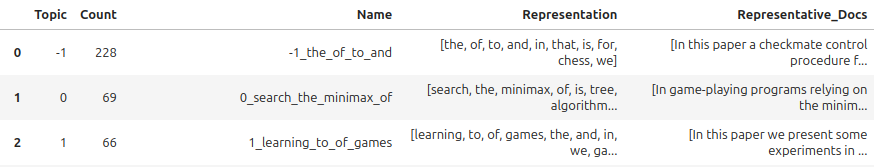
\includegraphics[width=1.0\textwidth]{img/img7.png}
    \caption{Porzione del dataset finale generato da BERTopic}
\end{figure}
Nonostante molteplici esecuzioni, adeguando le categorie descritte nel Paragrafo \ref{4.1}, BERTopic ha dimostrato difficoltà nell'assegnare argomenti predefiniti alla raccolta di documenti. Inoltre, come si evince dalla raffigurazione, alcuni di essi non sono stati nemmeno inclusi all'interno di un qualche insieme creato autonomamente dall'algoritmo. Una motivazione di tale comportamento, seppur marginale, potrebbe consistere nella mancata precisione del modello nel distinguere dati testuali che discutano temi simili o affini. Causa che potrebbe essere imputata all'impiego di una similarità per coseno, che non sempre riesce a catturare sottili differenze semantiche tra tematiche strettamente correlate. Pur di verificare la credibilità dell'ipotesi avanzata, nel Paragrafo \ref{4.4} è stato effettuato un ulteriore esperimento utilizzando documenti che trattassero argomenti differenti. \vspace{7pt} \\
Concludendo, per maggiore chiarezza, è riportata una tabella contenente delle brevi descrizioni delle colonne del dataset ottenuto da BERTopic.
\begin{table}[H]
    \begin{tabularx}{\textwidth}{|c|X|X|}
        \hline
        \small 1. & \small \textbf{Topic} & \small Identificatore numerico del topic \\
        \hline
        \small 2. & \small \textbf{Count} & \small Numero di documenti a cui è stato attribuito il topic \\
        \hline
        \small 3. & \small \textbf{Name} & \small Nome del topic, appartenente all'elenco predefinito oppure generato automaticamente dal modello \\
        \hline
        \small 4. & \small \textbf{Representation} & \small Lista delle parole chiave su cui si formalizza la correlazione tra documenti e topic \\
        \hline
        \small 5. & \small \textbf{Rapresentative Docs} & \small Lista dei documenti considerati rappresentativi per lo specifico topic \\
        \hline
    \end{tabularx}
    \caption{Tabella contenente le features del dataset ottenuto tramite BERTopic}
\end{table}

\section{Analisi degli esiti ottenuti dai modelli di linguaggio}
I modelli di linguaggio naturale implementati non hanno rispettato le aspettative. Pochissime osservazioni sono state correttamente classificate, testimoniando l'elevata difficoltà di etichettare le informazioni ricavate dall'insieme di documenti, mediante differenti liste predefinite di categorie (\ref{4.1}). \vspace{7pt} \\
Le tecniche di machine learning sviluppate sono state testate su diversi domini del dataset contenente le risorse in formato originale, ma indipendentemente dalle features utilizzate le etichettature finali non hanno mai evidenziato un netto miglioramento. In relazione agli esperimenti effettuati, sono stati impiegate le seguenti colonne:
\begin{itemize}
    \renewcommand{\labelitemi}{-}
    \item \textbf{Abstract}
    \item \textbf{Abstract + Introduction}
    \item \textbf{Title + Abstract + Introduction}
\end{itemize}
Seppur banale, è bene precisare che la categorizzazione secondo dati testuali più prolissi, come quelli indicati nell'elenco precedente, ha garantito annotazioni migliori rispetto a quanto sarebbe stato ottenuto tramite combinazioni relative ai titoli e alle keyword estratte, data la mancanza di informazioni al loro interno. Si ricorda che i modelli adottati sfruttano l'interpretazione del linguaggio naturale per adempiere a compiti di Natural Language Processing (NLP), pertanto adoperare dati testuali estesi, in grado di fornire le nozioni necessarie per la loro comprensione, aumenta la probabilità che gli esiti finali coincidano con quanto atteso. \vspace{7pt} \\
Prima di esprimere le cause che potrebbero aver influito sulla validità delle classificazioni, sono riportate alcune tabelle che descrivono l'andamento delle prove effettuate. Queste ultime mostreranno la superiorità di BART rispetto all'architettura GPT-4, sebbene non sia particolarmente marcata, e la ragione principale che ha spinto ad adeguare esclusivamente il primo modello a discapito del secondo.  
\begin{table}[H]
    \centering
    \begin{tabular}{l|cc|}
        \hline
        \textbf{Topic} & \textbf{Numero di articoli} \\
        \hline
        Algorithmic Approaches & 496 \\
        Architectural Designs & 0 \\
        Game Stages & 11 \\
        Traning and Evaluation & 0 \\
        Applications & 428 \\
        Ethical and Practical Concerns & 71 \\
        \hline
        \textbf{Non classificati} & 221 \\
    \end{tabular}
    \caption{Classificazione tramite GPT-4 secondo etichette di primo livello}
\end{table}
\begin{table}[H]
    \centering
    \begin{tabular}{l|cc|}
        \hline
        \textbf{Topic} & \textbf{Numero di articoli} \\
        \hline
        Algorithmic Approaches & 54 \\
        Architectural Designs & 0 \\
        Game Stages & 5 \\
        Traning and Evaluation & 12 \\
        Applications & 44 \\
        Ethical and Practical Concerns & 11 \\
        \hline
        \textbf{Non classificati} & 855 \\
    \end{tabular}
    \caption{Classificazione tramite BART secondo etichette di primo livello}
\end{table}
\begin{table}[H]
    \centering
    \begin{tabular}{l|l|c}
        \hline
        \textbf{Topic di Primo livello} & \textbf{Topic di Secondo livello} & \textbf{Numero di articoli} \\
        \hline
        & Search Techniques & 0 \\
        Algorithmic Approaches & Heuristics and Evaluation & 0 \\
        & Machine Learning & 9 \\
        \hline
        & Chess Engines & 6 \\
        Architectural Designs & Distributed Systems & 2 \\
        & Hardware & 1 \\
        \hline
        & Opening Play & 1 \\
        Game Stages & Middlegame Play & 2 \\
        & Endgame Play & 10 \\
        \hline
        & Data Sources & 0 \\
        Training and Evaluation & Benchmarks & 1 \\
        & Test Suites & 1 \\
        \hline
        & Competitive Play & 11 \\
        Applications & Education & 2 \\
        & Researh & 91 \\
        \hline
        & Cheating Prevention & 0 \\
        Ethical and Practical Concerns & Fairness in Play & 0 \\
        & Sustainability & 0 \\
        \hline
        & & \\
        \textbf{Non classificati} & & 844 \\
        & & \\
    \end{tabular}
    \caption{Classificazione tramite BART secondo etichette di secondo livello}
\end{table}
Come si può esaminare dai valori riportati, BART ha realizzato classificazioni più attendibili rispetto a GPT-4. In particolare, il Large Language Model ha mostrato una tendenza a omologare le annotazioni, privilegiando le categorie di carattere generale rispetto a classi più specifiche. Infatti, il modello sembra aver operato come se fosse stato "obbligato" ad assegnare un topic a ogni informazione testuale, ignorando sottili differenze semantiche e preferendo categorie il più possibile generali. Una causa di un comportamento simile potrebbe essere ricondotta alla natura generativa dei modelli LLM, i quali tendono a soddisfare la richiesta presentata creando una risposta probabilisticamente plausibile, rendendo la fase di classificazione inconsistente, soprattutto qualora le risorse manipolate presentano strutture testuali articolate e informazioni implicite. Alla luce di quanto emerso, l'opzione di classificazione secondo LLM è stata accantonata per gli esperimenti successivi. \vspace{7pt} \\
Contrariamente, i risultati ottenuti tramite BART sono stati più soddisfacenti, nonostante non siano stati raggiunti traguardi eccellenti. L'algoritmo, a differenza di GPT-4, ha dimostrato una maggiore capacità critica, adottando durante la classificazione non solo categorie generali, ma anche quelle più specifiche. Un fattore chiave di questa divergenza risiede nel processo di addestramento di BART, che si basa su un ampio corpus di documenti accademici. L'allenamento potrebbe aver contribuito allo sviluppo delle abilità fondamentali per l'interpretazione di contenuti semanticamente complessi, spesso caratterizzati dall'omissione di dettagli espliciti sulla tematica trattata. \vspace{7pt} \\
Per verificare se la categorizzazione fosse effettivamente problematica a causa delle etichette iniziali, sono stati introdotti \textbf{topic aggiuntivi}, ampliando il contesto dell'analisi. In questo modo, è stato possibile valutare se gli ostacoli presentati fossero legati alla specificità degli argomenti originali oppure ai limiti intrinseci del modello. Di seguito, sono fornite le classificazioni ottenute mediante l'impiego di due elenchi differenti di etichette. 
\begin{table}[H]
    \centering
    \begin{tabular}{l|cc|}
        \hline
        \textbf{Topic} & \textbf{Numero di articoli} \\
        \hline
        Historical Evolution of Computer Chess & 9 \\
        Famous Matches and Controversies & 4 \\
        Cognitive Science Insights & 7 \\
        Unsual Chess AI Strategies & 0 \\
        Failed Ideas in Computer Chess & 0 \\
        Alternative Chess variants and AI & 8 \\
        \hline
        \textbf{Non classificati} & 953 \\
    \end{tabular}
    \caption{Classificazione tramite BART secondo etichette relative a Entertainment}
\end{table}
\begin{table}[H]
    \centering
    \begin{tabular}{l|cc|}
        \hline
        \textbf{Topic} & \textbf{Numero di articoli} \\
        \hline
        Chess Playing & 487 \\
        Algorithms & 63 \\
        Hardware & 7 \\
        Machine Learning & 31 \\
        \hline
        \textbf{Non classificati} & 393 \\
    \end{tabular}
    \caption{Classificazione tramite BART secondo etichette relative alle quattro ere storiche}
\end{table}
La classificazione secondo etichette legate a temi di Entertainment in ambito computer chess ha nuovamente evidenziato l'inefficienza del modello pre-addestrato, che ha assegnato soltanto 26 categorie alle informazioni testuali recuperate. \vspace{7pt} \\
Sebbene BART avesse già mostrato prestazioni insufficienti nella categorizzazione secondo la lista di topic di primo e di secondo livello, si era comunque rivelato più affidabile rispetto al risultato ottenuto con GPT-4. Tuttavia, l'esito di questa fase conferma ulteriormente le sue limitazioni nell'elaborazione di dati testuali complessi. Una possibile spiegazione di quanto accaduto, potrebbe risiedere nell'impiego dello stesso insieme di etichette, caratterizzate da sfumature semantiche molto simili. Questa vicinanza concettuale potrebbe aver contribuito a una sovrapposizione delle categorie, riducendo così la capacità discriminativa del modello. \vspace{7pt} \\
Concludendo, anche l'ultima etichettatura non ha mostrato netti miglioramenti. In questa circostanza, BART ha omologato la classificazione, impiegando prevalentemente un'unica categoria. L'uso preponderante della classe \textbf{Chess Playing} potrebbe derivare dal fatto che le informazioni testuali appartengono ad articoli scientifici in ambito computer chess. Tuttavia, l'esperimento finale è stato condotto proprio per verificare se il modello di linguaggio fosse in grado di diversificare le classi, obiettivo che, dal quadro delineato, non è stato raggiunto.

\section{Esperimento sull'attendibilità di BERTopic}
\label{4.4}
La scarsità dei risultati ottenuti da BERTopic, ha suscitato alcune perplessità circa l'accuratezza delle informazioni ricavate. Pertanto, è stato sviluppato un ulteriore esperimento volto a identificare le potenziali criticità del modello e a confutare la credibilità dell'ipotesi avanzata al termine della Sezione \ref{4.2.3}: l'assenza di correlazioni tra i documenti e la lista predefinita di topic, potrebbe essere causata dall'impiego da parte dell'algoritmo di una similarità per coseno, inadeguata per operazioni in cui sia necessario catturare sottili differenze semantiche. \vspace{7pt} \\
Il flusso implementativo ricalca gli stessi passaggi illustrati nel paragrafo precedente, a differenza del fatto che il dataset non contiene solamente dati relativi agli articoli del caso di studio, ma si arrichisce di aggiuntive risorse inerenti a pubblicazioni scientifiche in ambito \textbf{quantum computing}. La scelta di combinare contenuti tra loro differenti è motivata dalla volontà di testare la correttezza della tecnica di machine learning, con l'obiettivo di ottenere una netta distinzione al termine dell'elaborazione. \vspace{7pt} \\
Il nuovo dataframe si compone di un totale di $80$ osservazioni, ciascuna completa in ogni feature; le entità aggiuntive sono state recuperate sfruttando la REST API di arXiv, selezionando casualmente $40$ lavori di ricerca in ambito di computazione quantistica.
\begin{lstlisting}[language=python, caption=Creazione e fitting del modello secondo il nuovo dataset]
list_topics = ["Computer Chess", "Quantum Computing"]

model = BERTopic(zeroshot_topic_list=list_topics, zeroshot_min_similarity=.6)
_topics, _ = model.fit_transform(docs, embeddings)
\end{lstlisting}
\begin{lstlisting}[language=python, caption=Recupero e visualizzazione del nuovo dataset finale generato da BERTopic]
df_new_bertopic = model.get_topic_info()
display(df_new_bertopic)
\end{lstlisting}
\begin{figure}[H]
    \centering
    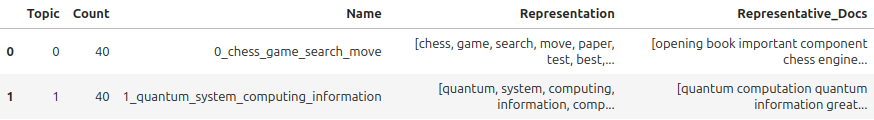
\includegraphics[width=1.0\linewidth]{img/img8.png}
    \label{4.2}
    \caption{Dataset finale generato da BERTopic}
\end{figure}
L'esito finale evidenzia una marcata divisione tra i due gruppi di documenti, valorizzando in questo modo la supposizione iniziale. Il modello BERTopic effettua attività di topic modeling soddisfacenti in casi in cui le informazioni adoperate possano essere contraddistinte in argomenti differenti e non correlati, manifestando quindi minori performance in circostanze in cui le informazioni possano essere ricondotte a molteplici tematiche.

\chapter{Conclusioni e sviluppi futuri}
\label{5.0}
I risultati ottenuti al termine dell'analisi hanno evidenziato numerose problematiche relative alla classificazione delle osservazioni recuperate secondo liste predefinite di etichette. Sebbene siano stati adeguati differenti accorgimenti durante la fase di estrazione di dati, i modelli di linguaggio naturale e di topic extraction non hanno mai restituito esiti considerati soddisfacenti. \vspace{7pt} \\
Durante lo sviluppo degli esperimenti è emerso un punto di debolezza comune per ogni algoritmo di apprendimento automatico utilizzato. In particolare, ciascuna tecnica implementata ha mostrato difficoltà nell'elaborazione di dati testuali complessi, soprattutto qualora il significato semantico delle informazioni contenute non era facilmente interpretabile. \vspace{7pt} \\
I modelli di linguaggio, infatti, pur essendo in grado di manipolare elevate quantità di testo, hanno mostrato significative vulnerabilità in circostanze in cui occorresse comprendere profondamente il tema trattato dal contenuto testuale. Inoltre, le annotazioni peggiori sono stati ottenute nei casi in cui la lista di etichette impiegata fosse caratterizzata da elementi concettualmente molto simili tra loro, in cui la capacità discriminativa dei modelli è diminuita drasticamente. \vspace{7pt} \\
Viceversa, gli strumenti attuati durante la fase di estrazione dei dati dall'insieme di articoli scientifici presi in esame, hanno garantito esiti più consistenti e affidabili, seppur con qualche difficoltà. GROBID e librerie Python per la lettura di file PDF, non hanno dimostrato la stessa efficacia nel manipolare il contenuto di file successivi ad una scansione rispetto a documenti creati digitalmente, scoraggiando l'estrapolazione di ulteriori dati. \vspace{7pt} \\
Nonostante gli obiettivi dichiarati dal caso di studio non siano stati completamente rispettati, le criticità emerse hanno evidenziato ulteriori opportunità di sviluppo. Ad esempio, l'incapacità degli strumenti attuali di gestire file scansionati suggerisce la possibilità di integrare meccanismi di Optical Character Recognition, in maniera tale che possano essere recuperate informazioni aggiuntive precedentemente impossibili da ricavare. In aggiunta, potrebbe essere considerata l'adozione di modelli fine-tuned su dataset specifici, concordi con le stesse tematiche trattate dalla collezione di pubblicazioni accademiche considerate, contribuendo a un miglioramento della comprensione e dell'interpretazione semantica. \vspace{7pt} \\
In sintesi, sebbene i risultati non abbiano pienamente soddisfatto le aspettative iniziali, le lacune individuate offrono una base solida per sviluppi futuri. Questa prospettiva permette non solo di colmare le attuali carenze, ma apre anche a nuove opportunità di ricerca e innovazione, rendendo la tesi presentata un punto di partenza piuttosto che un punto di arrivo.

\renewcommand{\bibsection}{}
\chapter*{Riferimenti bibliografici}
\bibliography{references}
\end{document}